\documentclass{article}	
% \usepackage[
%   height=2in,      % height of the text block
%   width=7in,       % width of the text block
%   top=100pt,        % distance of the text block from the top of the page
%   headheight=48pt, % height for the header block
%   headsep=30pt,    % distance from the header block to the text block
%                % ensure an integer number of lines
%            % show the values of the parameters in the log file
% ]{geometry}

\usepackage[margin=0.75in]{geometry}
\usepackage{fancyhdr}
\usepackage{duckuments}
\usepackage{enumitem}
\usepackage{graphicx}
\usepackage{tikz}
\usepackage[OT1]{fontenc}
\usetikzlibrary{automata,positioning}
\usetikzlibrary{shapes.geometric, arrows}
\usetikzlibrary{shapes.multipart}
\usetikzlibrary{calc, arrows.meta}
\usepackage{hyperref}
\usepackage{amssymb}
\usepackage{tikz}
\usepackage{bm}
\usepackage{tikz-3dplot}
\usetikzlibrary{calc,patterns}
\usetikzlibrary{arrows.meta, decorations.pathreplacing}
\usetikzlibrary{patterns}
\renewcommand{\familydefault}{\sfdefault}

\fancypagestyle{otherpages}{
    \fancyhf{}
    \fancyhead[LO]{MNBW2}
    \fancyhead[RO]{[MA9714]}
    \fancyfoot[RO]{Seite \thepage}
    \fancyfoot[LO]{Penguin}
}
\usepackage{amsmath}
\usepackage{lastpage} % To reference last page's number
\begin{document}
\begin{flushright}
    \includegraphics[width=2.3cm]{/home/penguin/Downloads/tum-logo/tum-logo.png} \\
\end{flushright}
\vspace{-1.5cm}
\noindent
\large 
\textcolor[HTML]{165DB1}{Mathematische Behandlung der Natur- und Wirtschaftswissenschaften 2
\\ Discrete Optimization \\ Department Mathematics}
\vspace{5mm}
\normalsize
\vspace{3mm}
\section{Basics of Ordinary Differential Equations (Grundlagen: Gewöhnliche Differentialgleichungen)}
\subsection{Solving a Differential Equation}
\textbf{Case 1: Homogeneous DE}\\[2mm]
we have: 
\hspace{10mm}$i(t) = 0$ \hspace{5mm}and
\hspace{5mm}$k'(t) = \delta k(t)$ \\[2mm]
\text{Claim: solution is} $k(t)=\gamma\cdot e^{\delta t}$ \newline
\text{Set of solutions for the homogeneous DE:} $\{\gamma\cdot e^{\delta t} : \gamma \in R\}$ \\[3mm]
\textbf{Case 2: Inhomogeneous DE} \hspace{5mm} we have a general $i(t)$ 
\begin{enumerate}
    \item It is sufficient to determine (particular) solution of the Inhomogeneous DE \newline
    $K_n(t) \rightarrow$ solution for the homogeneous DE $\Rightarrow$ $K'_n (t) = \delta \cdot K_n (t)$ 
    \newline
    $K_p(t) \rightarrow$ solution for the Inhomogeneous DE $\Rightarrow$ $K'_p(t) = \delta \cdot K_p (t) + i(t)$
    \newline combining both Equations, we have: \newline
    \begin{equation*}
    \begin{split} 
    K'(t) & = K'_p(t)+K'_n(t) \\
          & = \delta \cdot K_p(t) + i(t) + \delta \cdot K_n(t) \\
          & = \delta \cdot \left(K_p(t)+K_n(t)\right) + i(t) \\
          & = \delta \cdot K(t) + i(t)
    \end{split} 
    \end{equation*}
    \item \text{Determine one solution for Inhomogeneous DE through variation of constant} \newline
    $k(t) = \gamma \cdot e^{\delta t}$ \newline
    $k(t) = c(t) \cdot e^{\delta t}$ \newline
    substituting this into the DE  \\[1mm]
    \begin{equation} k'(t) = c'(t) \cdot e^{\lambda t} + c(t) \cdot \delta e^{\delta t} \end{equation}
    \begin{equation} k'(t) = k(t) \cdot \lambda + i(t) \end{equation} 
    from (1) and (2) we have:
    \begin{equation*} c'(t) \cdot e^{-\lambda \cdot t} = i(t) \end{equation*} \newline
    Integrating both sides 
    \hspace*{30mm} \begin{equation*}c(t) = \int {i(t) \cdot e^{-\lambda t}dt} \end{equation*}
    \vspace{5mm}
\end{enumerate}
\textbf{Example:} Solving an Ordinary Differential Equation
\begin{equation*} f'(x) = 1 - x + f(x), \hspace{1mm} f(0) = 2 \end{equation*} 
\begin{enumerate} 
    \item \text{Homogeneous DE:} 
    \begin{equation*}f'(x) = f(x) \Rightarrow f(x) = \gamma \cdot e^{x} \end{equation*}
    check: \begin{equation*} f'(x) = f(x) = \gamma \cdot e^{x} - \gamma \cdot e^{x} = 0 \end{equation*}
    \item \text{Variation of constant:} 
    \begin{equation*} f(x) = c(x) \cdot e^{x} \end{equation*}
    \begin{equation*} f'(x) = c'(x) \cdot e^{x} + c(x) \cdot e^{x} \end{equation*} 
    \begin{equation*} f'(x) - f(x) = 1 - x \end{equation*}  
    Replacing $f'(x)$ and $f(x)$ with the function of $c(x)$ and $c'(x)$
    \begin{equation*} c'(x) \cdot e^{x} + c(x) \cdot e^{x} - c(x) \cdot e^{x} = 1 - x \end{equation*} 
    \begin{equation*}  c'(x) = e^{-x} \cdot (1-x) \end{equation*}
    \begin{equation*}  c(x) = \int e^{-x} \cdot (1-x) dx \end{equation*}
    \begin{equation*}  c(x) = \int e^{-x} dx - \int e^{-x} \cdot x dx \end{equation*}
    \begin{equation*}  c(x) = e^{-x} \cdot x \end{equation*}
\text{Particular solution:} \begin{equation*} f(x) = c(x) \cdot e^{x} \Rightarrow f(x) = e^{-x} \cdot x \cdot e^{x} \end{equation*}
\begin{equation*} f(x) = x \Rightarrow f'(x) = 1 \end{equation*}
    \item \text{Set of solutions:} \newline
          \begin{equation*} f(x) = x + \gamma \cdot e^{x} \end{equation*}
    \item Initial Value: \begin{equation*} f(0) = 2 \end{equation*} 
         \begin{equation*} f(0) = 0 + \gamma = 2 \Rightarrow \gamma = 2 \end{equation*}
         \begin{equation*} \rightarrow  f(x) = x + 2 \cdot e^{x} \end{equation*}
         \text{solves the initial value problem}
\end{enumerate} 
\pagestyle{otherpages}
\textbf{Note: You can also solve the Differential Equation with the help of an integrating factor}\newline Refer to this wikipedia article \href{https://en.wikipedia.org/wiki/Integrating_factor}{integrating factor} and this \href{https://www.mathcentre.ac.uk/resources/uploaded/mathcentre-ode.pdf}{text}
\\[3mm]
\hspace*{70mm} \textbf{***} 
\subsection{System of Differential Equations}
A homogeneous system of Linear Differential Equations with constant coefficients is a system of the form: \\[2mm]
\begin{equation*}\begin{pmatrix} y'_1(t) \\ \vdots \\ \vdots \\ y'_n(t) \end{pmatrix} = A \cdot \begin{pmatrix} y_1(t) \\ \vdots \\ \vdots \\ y_n(t) \end{pmatrix}, \hspace{5mm} \begin{pmatrix} y_1(0) \\ \vdots \\ \vdots \\ y_n(0) \end{pmatrix} = \begin{pmatrix} \gamma_1 \\ \vdots \\ \vdots \\ \gamma_2 \end{pmatrix}\end{equation*} \\[2mm]
\hspace*{45mm} where A $\in R$ and $\begin{pmatrix} \gamma_1 \\ \vdots \\ \vdots \\ \gamma_2 \end{pmatrix} \in R^{n} $ \\[2mm]
The key idea is that if A is a diagonal matrix, then each row is a Differential Equation that is independent of the others, solve each row separately \textbf{decoupled system}
\begin{equation*} \begin{pmatrix} y'_1(t) \\ y'_2(t) \end{pmatrix} = \begin{pmatrix} \lambda_1 & 0 \\ 0 & \lambda_2 \end{pmatrix} \begin{pmatrix} y_1(t) \\ y_2(t) \end{pmatrix}  \end{equation*}
We need a basis and a corresponding basis transformation S $\in R^{n \times n}$ such that $S^{-1}AS = D$ is diagonal \newline
Then we substitute, y = SZ $\Rightarrow Z = S^{-1}y$ \newline
The DE system, \begin{equation*} y' = A \cdot y \end{equation*} 
becomes \begin{equation*} S \cdot z = A \cdot S \cdot Z \end{equation*} 
\begin{equation*} Z' = S^{-1} \cdot A \cdot S \cdot Z = D \cdot Z \end{equation*}
Solve the new decoupled system and transform solution back through $y = SZ$ \newline
\textbf{Example:} 
\begin{equation*} \gamma'(t) = \frac{5}{2} \cdot \gamma(t) - \phi(t) \end{equation*}
\begin{equation*} \phi'(t) = \frac{-1}{4} \cdot \gamma(t) + \frac{5}{2} \phi(t) \end{equation*}
matrix form \begin{equation*} \begin{pmatrix} \gamma' \\[6pt] \phi' \end{pmatrix} = \begin{pmatrix} \dfrac{5}{2} & -1 \\[9pt] \dfrac{-1}{4} & \dfrac{5}{2} \end{pmatrix} \begin{pmatrix} \gamma \\[6pt] \phi \end{pmatrix}\end{equation*}
now, determine the eigenvalues and eigenvectors for the matrix\newline
\begin{equation*} p_A(\lambda) = \det(A-\lambda I_2) = \det\begin{pmatrix} \dfrac{5}{2} - \lambda & -1 \\[9pt] \dfrac{-1}{4} & \dfrac{5}{2} - \lambda \end{pmatrix} = {\left(\frac{5}{2}-\lambda\right)}^{2} - \frac{1}{4} = \frac{25}{4} + \lambda^{2} - 5\lambda - \frac{1}{4} = 6 + \lambda^{2} -5\lambda = (\lambda-3)(\lambda-2) \end{equation*}
The roots of the equation are $\lambda_1 = 3$ and $\lambda_2 = 2$ \newline
For the respective eigenspaces, we get \newline
\begin{equation*} eig_A(3) = \ker(A-3I_2) = \ker\begin{pmatrix} \dfrac{-1}{2} & -1 \\[9pt] \dfrac{-1}{4} & \dfrac{-1}{2}\end{pmatrix} = \ker\begin{pmatrix} \dfrac{1}{2} & -1 \\[9pt] 0 & 0\end{pmatrix} = span\begin{Bmatrix}\begin{pmatrix} -2 \\1 \end{pmatrix}\end{Bmatrix} \end{equation*}
\begin{equation*} eig_A(2) = \ker(A-2I_2) = \ker\begin{pmatrix} \dfrac{1}{2} & -1 \\[9pt] \dfrac{-1}{4} & \dfrac{1}{2}\end{pmatrix} = \ker\begin{pmatrix} \dfrac{1}{2} & -1 \\[9pt] 0 & 0\end{pmatrix} = span\begin{Bmatrix}\begin{pmatrix} 2 \\1 \end{pmatrix}\end{Bmatrix} \end{equation*}
\begin{equation*} S = \begin{pmatrix} -2 & 2 \\ 1 & 1 \end{pmatrix}\end{equation*}
\begin{equation*} S^{-1} = \frac{-1}{4}\begin{pmatrix} 1 & -2 \\ -1 & -2 \end{pmatrix}\end{equation*}
\begin{equation*} S^{-1}AS = \begin{pmatrix} 3 & 0 \\ 0 & 2 \end{pmatrix} = D \end{equation*}
Solve the system: \begin{equation*} Z' = DZ = \begin{pmatrix} 3 & 0 \\ 0 & 2 \end{pmatrix} \end{equation*}
\begin{equation*} Z_1(t) = \gamma_1 e^{3t} \end{equation*}
\begin{equation*} Z_2(t) = \gamma_2 e^{2t} \end{equation*}
\\[2mm]
\begin{equation*} \begin{pmatrix} \gamma \\[6pt] \phi  \end{pmatrix} = \begin{pmatrix} -2 & 2 \\[6pt] 1 & 1 \end{pmatrix} \begin{pmatrix} \gamma_1 e^{3t} \\[6pt] \gamma_2 e^{2t} \end{pmatrix} \end{equation*}
\begin{equation*} \gamma(t) = -2 \gamma_1 e^{3t} + 2 \gamma_2 e^{2t} \end{equation*}
\begin{equation*} \phi(t) = \gamma_1 e^{3t} \gamma_2 e^{3t} \end{equation*}
we know the initial values: $\gamma(0) = 60$ and $\phi(0) = 60$ \newline
\begin{equation*} -2\gamma_1 + 2\gamma_2 = 60\end{equation*}
\begin{equation*} \gamma_1 + \gamma_2 = 60 \end{equation*} 
solving, we get $\gamma_1 = 15$ and $\gamma_2 = 45$
\begin{equation*} \gamma(t) = -30 e^{3t} + 90 e^{2t} \end{equation*}
\begin{equation*} \phi(t) = 15 e^{3t} + 45 e^{2t} \end{equation*}
\normalsize
\pagestyle{otherpages}
\subsection*{Basics of Complex Numbers}
A complex number is represented as $Z = a + i b$ where a and b are real numbers and \begin{equation*} Re(Z)=a \end{equation*} \begin{equation*} Im(Z)=b \end{equation*}
\begin{equation*} i = \sqrt{-1} \end{equation*}
\begin{equation*} i^{2} = -1 \end{equation*}
A complex number can be represented on an argand plane with the X-axis as the real part of the complex number and the Y-part as the imaginary part of the complex number\\[2pt]
\
\subsubsection*{Algebra of Complex numbers}
Two complex numbers $Z_1 = a_1 + i b_1$ and $Z_2 = a_2 + i b_2$ can be added and subtracted by seperately adding/subtracting their real and imaginary parts. \\
Multiplication of two complex numbers,
\begin{equation*} Z_1 \cdot Z_2 = a_1 a_2 + i a_1 b_2 + i b_1 a_2 + i^{2} b_1 b_2 = a_1 a_2 + i (a_1 b_2 + b_1 a_2) - b_1 b_2  \end{equation*}
Division of two complex numbers, \\
Mulitiplying both numerator and denominator by the \textbf{conjugate} of the denominator inorder to obtain a real denominator and a complex numerator.
For example,
\begin{equation*} \frac{4+3i}{1+2i} = \frac{(4+3i)(1-2i)}{(1+2i)(1-2i)} = \frac{4-8i+3i-6i^2}{1-4i^2} = \frac{12+5i}{5} = \frac{12}{5} + i \end{equation*}
\subsection*{Complex Conjugate and absolute value}
For a complex number $Z = a + ib$, the complex conjugate is defined as $\overline{Z} = a - ib$ 
\begin{equation} Z\overline{Z} = (a+ib)(a-ib) = a^{2} - i ab + i ab + b^{2} = a^{2} + b^{2}\end{equation}
As per the definition of the absolute value of a complex number
\begin{equation} |Z| = \sqrt{a^2 + b^2} \end{equation} 
By (1) and (2), we have
\begin{equation*} Z\overline{Z} = |Z|^{2} \end{equation*}
\subsection*{Polar form and Euler's form}
Representing the complex number in the form of a $|Z|$ and argument $\phi$ 
\begin{equation*} Z = |Z| (\cos\phi+i \sin\phi)\end{equation*} is the Polar representation of a complex number
\begin{equation*} e^{i \phi} = \cos\phi + i \sin \phi \end{equation*}
Therefore, 
\begin{equation*} Z = |Z| e^{i \phi} \end{equation*} is the Euler form of the complex number 
A lot of cool stuff related to \href{https://www.youtube.com/playlist?list=PLJbzH0qGCsyrO7lUmdEQAzJInNlwwUgp0}{complex number} on this playlist. Not required for economic aspects though.
\section{Eigenvectors and Eigenalues (Eigenwertprobleme)} 
$S \in R^{n\times n}$ \\
$A \in R^{n \times n}$ \\
$S^{-1}AS = D$ diagonal matrix, tranformation matrix \\
Is there a basis transformation? \\ 
$\lambda \in R$ is called an eigenvalue of A if there exists a vector $v \neq \phi$ such that \begin{equation*} A \cdot v = \lambda \cdot v \end{equation*}
Any such vector v in this case would be called an eigen vector of A for the eigen value $\lambda$
\textbf{Gaussian Reformulation:} Determination of the eigenvalues and eigenvectors. \\
$\lambda$ is an eigenvalue of A if there $v\neq\phi$ with $A\cdot v = \lambda \cdot v$
\begin{equation*}
    \Leftrightarrow A\cdot v - \lambda \cdot v = 0 \end{equation*}
\begin{equation*}\Leftrightarrow (A-\lambda E_n) \cdot v = 0 \end{equation*}
\begin{equation*} \Leftrightarrow v \in \ker(A\cdot\lambda E_n) \end{equation*}
\begin{equation*}\Leftrightarrow (A-\lambda E_n) \text{  is not invertible} \end{equation*}
\begin{equation*} \Leftrightarrow \det(A-\lambda E_n) = 0 
\end{equation*} \\[2pt]
The \textbf{characteristic polynomial} $p_A(\lambda)$ is defined as the determinant $\det(A-\lambda E_n)$ \begin{equation*} p_A(\lambda) = \det(A-\lambda E_n) \end{equation*} \\ and the kernel $\ker(A-\lambda E_n)$ is called the \textbf{eigenspace of A for the eigenvalue $\lambda$} and written as \begin{equation*} eig_A(\lambda) = \ker(A-\lambda E_n) \end{equation*}
The idea to solve each and every problem here is quite simple,
\begin{enumerate}
    \item First of all, determine the \textbf{characteristic polynomial} [Diagonalized matrix S is the matrix with the eigenspaces of the respective eigenvalues]
    \item Find the roots of the characteristic polynomial, these are the eigenvalues of A
    \item For each eigenvalue of A, determine the eigenspace by solving the linear equation system \\ $(A-\lambda E_n) \cdot v = 0$ 
\end{enumerate}
\subsection{Diagonalization using complex numbers} 
characterizing which matrices can be transformed into diagonal form, ie possess an eigenvector basis. \\
A matrix $A\in R^{n\times n}$ is called \textbf{diagonalizable} if there is a basis of $R^{n}$ that consists of eigenvectors of A\\[2pt]
\underline{NOTE:} For each eigenvalue $\rightarrow$ there is at least one eigenvector ie. $\dim(eig_A(\lambda)) \geq 1$ for each eigenvalue $\lambda$ 
$\Rightarrow$ if A possesses n distinct eigenvalue, then there are at least n eigenvectors \\
\begin{equation*} p_A(\lambda) = {(\lambda - \lambda*)}^k \cdot g(\lambda) \text{   and  } g(\lambda*) \neq 0 \end{equation*}
Then k is called the \textbf{algebraic multiplicity} of $\lambda*$ and $\dim(eig_A(\lambda*))$ is called the geometric mutliplicity of $\lambda*$
\begin{enumerate}
    \item Algebraic mulitplicity $\geq$ Geometric mulitplicity
    \item For pairwise distinct eigenvalues of A with corresponding eigenvectors- the set $\{v_1, \dots, v_r\}$ is linearly independent
    \item For a matrix to be diagonalizable, the algebraic and the geometric mulitplicity have to be equal for every eigenvalue of A 
\end{enumerate}
Proving (2) is pretty simple as you can simply use the principle of induction after solving it for 2 eigenvalues and their corresponding eigenvectors
\\ If roots are complex, we can use the Euler's formula \begin{equation*} e^{i \phi} = \cos\phi + i \sin \phi \end{equation*}
what if the matrix cannot be diagonalized? \textbf{JORDAN NORMAL FORM} as \href{https://en.wikipedia.org/wiki/Jordan_normal_form}{generalizations} and refer \href{https://shorturl.at/9Vxni}{for} Inhomogeneous Differential Equation system 
\\\url{https://people.math.harvard.edu/~knill/teaching/math19b_2011/handouts/lecture29.pdf} for a recap
\subsection{Predator-Prey Model}
squirrels-hawks $\rightarrow$ The growth of hawk population depends on availability of squirrels and vice-versa. [Fewer hawks $\rightarrow$ higher the growth rate of squirrels]
\\ Model this through DE system:
\begin{equation*} h'(t) = s(t) - 12 \text{ and } h(0) = 6\end{equation*}
\begin{equation*} s'(t) = -h(t) \text{  and  } s(0) = 20 \end{equation*}
\begin{enumerate} 
    \item \underline{get rid of constants:} define a new system \\
    \begin{equation*} y_1(t) = h(t) - 10 = -s'(t) \text{    and    } y_1(0) = h(0) - 10 = -4\end{equation*}
    \begin{equation*} y_2(t) = s(t) - 12 = h'(t) \text{   and   }  y_2(0) = s(0) - 12 = 8 \end{equation*}
    \begin{equation*} \Rightarrow y_1'(t) = h'(t) = s(t) - 12 = y_2(t)  \end{equation*}
    \begin{equation*} \Rightarrow y_2'(t) = -h(t) + 10 \end{equation*} 
    \text{new system without constants:} 
    \begin{equation*} \begin{pmatrix} y_1'(t) \\ y_2'(t) \end{pmatrix} = \begin{pmatrix} 0 & 1 \\ -1 & 0 \end{pmatrix} \begin{pmatrix} y_1(t) \\ y_2(t) \end{pmatrix} \mid \begin{pmatrix} y_1(0) \\ y_2(0) \end{pmatrix} = \begin{pmatrix} -4 \\ 8 \end{pmatrix} \end{equation*} 
    \item \underline{Diagonalize the matrix A} [find eigenvalues and the corresponding eigenvectors then form the S matrix]\begin{equation*} A = \begin{pmatrix} 0 & 1 \\ -1 & 0 \end{pmatrix} \end{equation*}
    not showing the calculations but the eigenvectors are $+i$, $-i$ and eigenvectors are $\begin{pmatrix} 1 \\ i \end{pmatrix}$ and $\begin{pmatrix} 1 \\ -i \end{pmatrix}$ so the required S matrix is $\begin{pmatrix} 1 & 1 \\ i & -i \end{pmatrix}$ \\
    \begin{equation*} S^{-1}AS = \begin{pmatrix} i & 0 \\ 0 & -i \end{pmatrix} \end{equation*}
    \item \underline{consider the decoupled system after substitution} $y=SZ$ \\
    \begin{equation*} Z'(t) = \begin{pmatrix} i & 0 \\ 0 & i \end{pmatrix} Z(t)\end{equation*}
    $\Rightarrow$
    \begin{equation*} Z_1'(t) = i\cdot Z_1(t) \Rightarrow Z_1(t) = \gamma_1 \cdot e^{i t} \end{equation*}
    \begin{equation*} Z_2'(t) = -i \cdot Z_2(t) \Rightarrow Z_2(t) = \gamma_2 \cdot e^{-i t} \end{equation*}
    \item \underline{determine y = SZ:} \begin{equation*} y(t) = \begin{pmatrix} 1 & 1 \\ i & -i \end{pmatrix} \begin{pmatrix} \gamma_1 e^{i t} \\ \gamma_2 e^{-i t} \end{pmatrix}\end{equation*}  
    $\Rightarrow$
    \begin{equation*} y_1(t) = \gamma_1 e^{i t} + \gamma_2 e^{-i t} \end{equation*}
    \begin{equation*} y_2(t) = \gamma_2 i e^{i t} - \gamma_2 i e^{-i t} \end{equation*} 
    \item \underline{Determine $\gamma_1$, $\gamma_2$ through initial values:}
    \begin{equation*} y_1(0) = -4 = \gamma_1 \cdot 1 + \gamma_2 \cdot 1 \end{equation*}
    \begin{equation*} y_2(0) = 8 = \gamma_1 \cdot i \cdot 1 - \gamma_2 \cdot i \cdot 1 \end{equation*}
    \begin{equation*} \rightarrow \begin{pmatrix} 1 & 1 &\bigm| & -4 \\  i & -i &\bigm| & 8  \end{pmatrix} \rightarrow \begin{pmatrix} 1 & 1 &\bigm| & -4 \\ 0 & -2i &\bigm| & 8+4i \end{pmatrix} \end{equation*}
    \begin{equation*} (-2i) \gamma_2  = 8 + 4 i \end{equation*}
    \begin{equation*} \Leftrightarrow \gamma_2 = 4i - 2 = -2 + 4i \end{equation*} 
    \begin{equation*} \Rightarrow \gamma_1 = -4 - \gamma_2 = -2 - 4i \end{equation*}
    \textbf{Solutions:}
    \begin{equation*} y_1(t) = (-2 - 4i) e^{i t} + (-2 + 4i) e^{-i t} \end{equation*} 
    \begin{equation*} y_2(t) = (4 - 2i) e^{i t} + (4 + 2i) e^{-i t} \end{equation*}
    \item \underline{Use Euler's Formula:} replace $e^{i t}$ and $e^{-i t}$ with $cis\theta$ terms
    \begin{equation*} y_1(t) = -4\cos t + 8\sin t \mid h(t) = -4\cos t + 8\sin t + 10\end{equation*}
    \begin{equation*} y_2(t) = 8\cos t + 4\sin t \mid s(t) = 8\cos t + 4\sin t + 12 \end{equation*}
\end{enumerate} \vspace{10mm}
\section{Multivariable Calculus}
\subsection{Fundamentals}
\textbf{Definition:} Let $f : X \rightarrow Y$ be a function with $ X \subseteq \mathbb{R}^{n} $ (domain) and $ Y \subseteq \mathbb{R}^{n} $ (codomain) for $m, n \in \mathbb{N}$ \\
The graph of $f$ is the set 
\begin{equation*} graph(f) = \left\{\begin{pmatrix} x \\ f(x)\end{pmatrix} :  x \in X \right\} \end{equation*}
A function of two variables assigns a real number to each point in a subset of $\mathbb{R}^2$. For example,
\[
f(x, y) = x^2 + y^2
\]
defines a function over $\mathbb{R}^2$.
The \textbf{domain} of a multivariable function is the set of all input values for which the function is defined. The \textbf{range} is the set of all output values.
Example: For $f(x, y) = \sqrt{1 - x^2 - y^2}$, the domain is the unit disk:
\[
D = \{(x, y) \in \mathbb{R}^2 : x^2 + y^2 \leq 1\}
\]
\textbf{Definition:} Let $f : X \rightarrow \mathbb{R}$, $ X \subseteq \mathbb{R}^{n} $ be a function and let $\gamma \in \mathbb{R}$ \\ 
The set 
\begin{equation*} L_{f} (\gamma) := \left\{x \in X : f(x) = \gamma \right\}\end{equation*} is called the \underline{level set of $f$ for level $\gamma$}
\newpage 
\subsection{Basic Topology}
\subsubsection{Open Balls and $\delta$-Neighborhoods}
Let $x^{*} \in \mathbb{R}^n$, $\delta > 0$. Then the $\delta$-neighborhood of $x^{*}$ is the set
\[
N_{\delta} (x^{*}) := \left\{x \in \mathbb{R}^{n}: ||x - x^{*}|| < \delta\right\}
\]
for some $\delta > 0$. $N_{\delta}$ is called \textbf{open ball of radius $\delta$ around $x^{*}$ and sometimes denoted by $B_{\delta}(x^{*}$)} 

\subsubsection{Interior Points}
A point $x \in A \subseteq \mathbb{R}^n$ is called an \textbf{interior point} of $A$ if there exists a $\delta > 0$ such that:
\[
N_{\delta} (x*) \subseteq X
\]
The set of all interior points of $X$ is called the \textbf{interior} of $X$, denoted $\operatorname{int}(X)$.

\subsubsection{Boundary Points}
A point $x \in \mathbb{R}^n$ is a \textbf{boundary point} of a set $A$ if every $\delta$-neighborhood of $x$ intersects both $X$ and its complement (not in $X$):
\[
\forall \delta > 0,\ N_\delta(x^{*}) \cap X \neq \emptyset \quad \text{and} \quad N_\delta(x^{*}) \cap (\mathbb{R}^n \setminus X) \neq \emptyset
\]
The set of all boundary points is called the \textbf{boundary} of $X$, denoted $bd(X)$ or $\partial X$.
\\ 
The set $cl(X) := X \cup bd(X)$ is called \textbf{closure} of $X$ (sometimes written $\bar{X}$)
\subsubsection{Closure of a Set}
The \textbf{closure} of a set $X$, denoted $\overline{X}$, is the union of $X$ and its accumulation points. Equivalently,
\[
\overline{X} = X \cup \partial X
\]
\subsubsection{Open and Closed Sets}
\begin{enumerate} \item A set $A$ is \textbf{open} if all its points are interior points, i.e., $A = \operatorname{int}(A)$.
\item A set is \textbf{closed} if it contains all its boundary points.
\end{enumerate}
\subsubsection{Accumulation (Limit) Points}
A point $x$ is an \textbf{accumulation point} (or limit point) of a set $X$ if every neighborhood of $x$ contains at least one point of $X$ different from $x$:
\[
\forall \delta > 0, \quad (B_\delta(x) \setminus \{x\}) \cap X \neq \emptyset
\]
\newpage 
The set $X$ is called 
\begin{enumerate}
    \item \textbf{open} if $X = int(X)$
    \item \textbf{closed} if $\mathbb{R} \setminus X$ is open 
    \item \textbf{bounded} if there is some $\delta > 0$ such that $X \subseteq N_{\delta}(0)$
    \item \textbf{compact} if it is closed and bounded.
\end{enumerate} \vspace{10mm}
    1. $\delta$-Neighborhood (Open Ball)
\begin{center}
    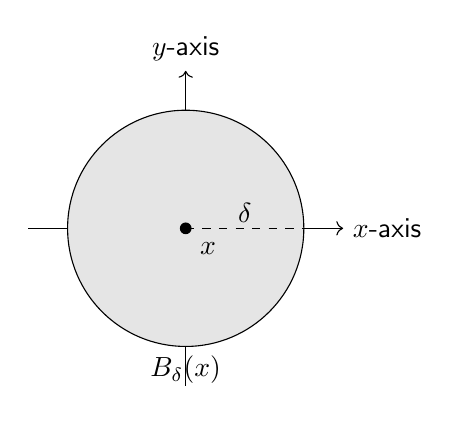
\begin{tikzpicture}
      \draw[->] (-2,0) -- (2,0) node[right] {$x$-axis};
      \draw[->] (0,-2) -- (0,2) node[above] {$y$-axis};
    
      \filldraw[fill=gray!20, draw=black] (0,0) circle (1.5);
      \node at (0,0) [circle,fill,inner sep=1.5pt,label=below right:$x$] {};
    
      \draw[dashed] (0,0) -- (1.5,0);
      \node at (0.75,0.2) {$\delta$};
      \node at (0,-1.8) {$B_\delta(x)$};
    \end{tikzpicture}
    \end{center}
    \vspace{5mm}
    2. Interior Point
    \begin{center}
    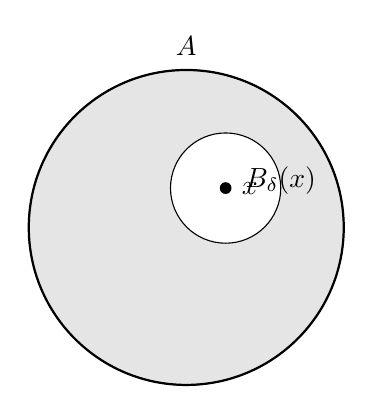
\begin{tikzpicture}
      \draw[fill=gray!20] (0,0) circle (2);
      \draw[thick] (0,0) circle (2);
      \node at (0,2.3) {$A$};
    
      \filldraw[fill=white,draw=black] (0.5,0.5) circle (0.7);
      \node at (0.5,0.5) [circle,fill,inner sep=1.5pt,label=right:$x$] {};
      \node at (1.2,0.6) {$B_\delta(x)$};
    \end{tikzpicture}
    \end{center}
    \vspace{5mm}
    3. Boundary Point
    \begin{center}
    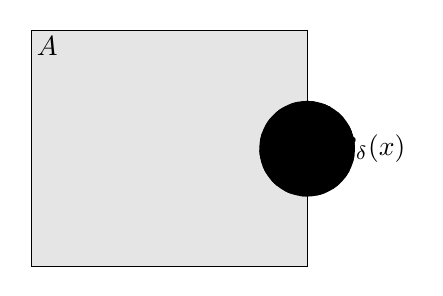
\begin{tikzpicture}
      \draw[fill=gray!20] (-2,-1) rectangle (1.5,2);
      \node at (-1.8,1.8) {$A$};
    
      \filldraw[draw=black] (1.5,0.5) circle (0.6);
      \node at (1.5,0.5) [circle,fill,inner sep=1.5pt,label=above:$x$] {};
      \node at (2.3,0.5) {$B_\delta(x)$};
    
      \draw[dashed] (1.5,0.5) circle (0.6);
    \end{tikzpicture}
    \end{center}
    \vspace{50mm}
    4. Closed Set
    \begin{center}
    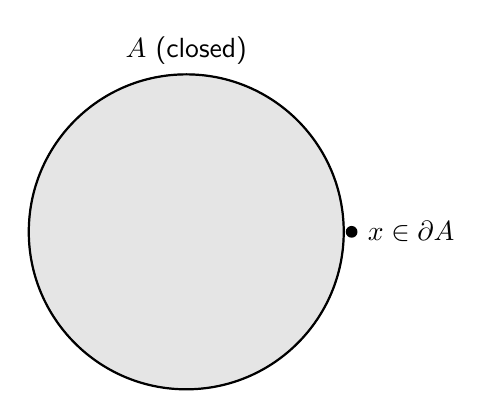
\begin{tikzpicture}
      \draw[fill=gray!20] (0,0) circle (2);
      \draw[thick] (0,0) circle (2);
      \node at (0,2.3) {$A$ (closed)};
      \node at (2.1,0) [circle,fill,inner sep=1.5pt,label=right:$x \in \partial A$] {};
    \end{tikzpicture}
\end{center}
    \vspace{5mm}
    5. Open Set
    \begin{center}
    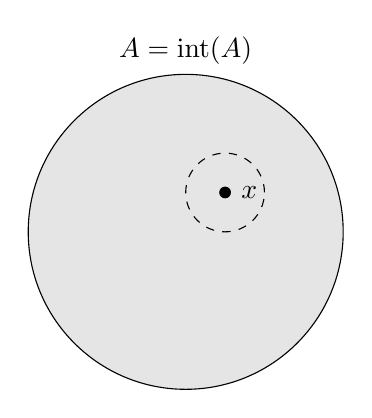
\begin{tikzpicture}
      \draw[fill=gray!20] (0,0) circle (2);
      \node at (0,2.3) {$A = \operatorname{int}(A)$};
      \node at (0.5,0.5) [circle,fill,inner sep=1.5pt,label=right:$x$] {};
      \draw[dashed] (0.5,0.5) circle (0.5);
    \end{tikzpicture}
\end{center} \vspace{10mm}
\subsection{Sequences and Limits}
A function in $f : \mathbb{N}_{0} \rightarrow \mathbb{R}^n$ is called a \textbf{sequence} in $\mathbb{R}^{n}$ with $a_k := f(k)$ such a sequence is usually \\ denoted as $(a_k)_{k \in \mathbb{N}_{0}}$ or just $(a_k)_{\mathbb{N}_{0}}$ 
\\
A sequence $(a_k)_{\mathbb{N}}$ is called \textbf{convergent} if there exists a vector $a \in \mathbb{R}^n$ such that
\[
\forall \varepsilon > 0, \ \exists N \in \mathbb{N} \text{ such that } ||a_k - a|| \rightarrow 0 
\]
as $k \rightarrow \infty$. The vector a is called the \textbf{limit of $(a_k)_{\mathbb{N}}$} and is denoted by \begin{equation*} a = \lim a_k\end{equation*}
$(a_k)_{\mathbb{N}}$ is convergent with limit $a$ if and only for $i = 1, \dots, n$ the following holds:
\begin{enumerate}
    \item the sequence $(\alpha_ik)_{k \in \mathbb{N}}$ is convergent
    \item $\lim_{k} \alpha_{ik} = \alpha_{i}$
\end{enumerate} \newpage
\textbf{Definitions}
\begin{enumerate}
\item A sequence $\{a_k\} \subset \mathbb{R}^n$ is \textbf{bounded} if the set $\left\{a_k : k \in \mathbb{N}_{0}\right\}$ is bounded
\item Let $(a_k)_{\mathbb{N}_{0}}$ be a sequence and $f : \mathbb{N}_{0} \rightarrow \mathbb{N}_{0}$ be strictly increasing, i.e. for $p > q \implies f(p) > f(q)$. \\ Then the sequence $(a'_k)_{\mathbb{N}_{0}}$ defined as $a'_k = a_{f(k)}$ is called a \textbf{subsequence} of $(a_k)_{\mathbb{N}_{0}}$ 
\item The limit of a convergent subsequence of some sequence $(a_k)_{\mathbb{N}_{0}}$ is called the \textbf{accumulation point} of $(a_k)_{\mathbb{N}_{0}}$ 
\end{enumerate}
\subsubsection{Bolzano-Weierstrass Theorem}
\textbf{Theorem:} Every bounded sequence in $\mathbb{R}^n$ has a convergent subsequence. (i.e. at least one accumulation point) \\
in particular, if $X$ is a compact set and  $(a_k)_{\mathbb{N}_{0}}$ is a subsequence in $X$, then  $(a_k)_{\mathbb{N}}$ has a convergent subsequence with limit in $X$.
\\ 
\textit{Idea of Proof:} Use the fact that $\mathbb{R}^n$ is a product of complete metric spaces, and apply the one-dimensional Bolzano-Weierstrass theorem component-wise to extract a convergent subsequence.
\vspace{10mm}
\subsection{Continuity}

\textbf{Definition:}\\
Let \( X \subseteq \mathbb{R}^m \), \( f: X \rightarrow \mathbb{R}^m \) and \( x^* \in X \).

\begin{enumerate}
    \item[(3)] \(\alpha \in \mathbb{R}^m\) is called the limit of \( f \) for \( x \rightarrow x^* \) if the following holds:
    
    For every sequence \((a_k)_{k \in \mathbb{N}}\) in \( X \) that converges to \( x^* \), the sequence \((f(a_k))_{k \in \mathbb{N}}\) converges to \(\alpha\).
    
    \[
    \lim_{x \rightarrow x^*} f(x) = \alpha
    \]
    
    \item[(2)] \( f \) is called continuous in \( x^* \) if 
    
    \[
    \lim_{x \rightarrow x^*} f(x) = f(x^*).
    \]
    
    \item[(3)] \( f \) is called continuous on \( X \) if \( f \) is continuous at every point \( x^* \in X \).
\end{enumerate}

\subsubsection{Theorem:}
Let \( X \subseteq \mathbb{R}^m \), \( f: X \rightarrow \mathbb{R}^m \) and \( g: X \rightarrow \mathbb{R} \) be continuous on \( X \), and let \( \alpha \in \mathbb{R} \). Then the following are true:

\begin{enumerate}
    \item[(1)] \( f + g \), \( \alpha f \), and \( f \cdot g \) are continuous on \( X \).
    
    \item[(2)] \(\frac{f}{g}\) is continuous on \( X \setminus \{ x \in X : g(x) = 0 \}\).
    
    \(\frac{f}{\alpha}\) is continuous for \( \alpha \neq 0 \).
    
    \item[(3)] Let \( h: \mathbb{R}^k \rightarrow X \) be continuous, then \( f \circ h \) is continuous.
    
    \item[(4)] If 
    \[
    f(x) = \begin{pmatrix}
    f_1(x) \\
    \vdots \\
    f_m(x)
    \end{pmatrix},
    \]
    then \( f \) is continuous on \( X \) if and only if all \( f_i: X \rightarrow \mathbb{R} \) are continuous on \( X \).
\end{enumerate}

\subsubsection*{Example:}
\[
f(x_1, x_2) := \begin{pmatrix}
x_1 \cos(x_2) \\
e^{x_1 + x_2} - 1
\end{pmatrix}, \quad f: \mathbb{R}^2 \rightarrow \mathbb{R}^2.
\]

Then \( f \) is continuous:

\begin{enumerate}
    \item[(1)] \( f \) is continuous if and only if both coordinate functions are continuous:
    \[
    f_1(x_1, x_2) = x_1 \cos(x_2), \quad f_2(x_1, x_2) = e^{x_1 + x_2} - 1.
    \]
    
    \item[(2)] \( f_1 \) is a product of continuous functions, hence continuous.
    
    \item[(3)] \( f_2 \) is the sum of continuous functions. The term \( e^{x_1 + x_2} \) is continuous as it is a composition of continuous functions.
    
    \(\Rightarrow f_2 \) is continuous.
\end{enumerate}

\subsubsection*{Definition:}
A multivariate polynomial is a function \( p: \mathbb{R}^n \rightarrow \mathbb{R} \) of the form:
\[
p(x) = \sum_{I} a_I x^I,
\]
where \( I \) is a multi-index and \( a_I \in \mathbb{R} \).

\subsubsection*{Example:}
\[
p(x_1, x_2, x_3) = 2x_1^2 + 4x_2^3 + 8x_3^4.
\]

Multivariate polynomials are continuous on \( \mathbb{R}^n \).

\begin{enumerate}
    \item[(1)] Sum of simple functions (monomials).
    \item[(2)] Each monomial is a product of constants and univariate monomials.
    \item[(3)] Products and sums of continuous functions are continuous.
\end{enumerate}

\subsubsection{Theorem:}
Let \( X \subseteq \mathbb{R}^n \), \( f: X \rightarrow \mathbb{R}^m \). Then \( f \) is continuous if and only if:

\begin{enumerate}
    \item[(i)] For any open set \( Y \subseteq \mathbb{R}^m \), the preimage \( f^{-1}(Y) \) is open in \( X \).
    \item[(ii)] For every closed set \( Y \subseteq \mathbb{R}^m \), the preimage \( f^{-1}(Y) \) is closed in \( X \).
\end{enumerate}

\subsubsection{Theorem:}
Let \( X \subseteq \mathbb{R}^n \), \( f: X \rightarrow \mathbb{R}^m \) continuous. If \( X \) is compact, then \( f(X) \) is also compact (closed and bounded).

This implies: For compact \( X \subseteq \mathbb{R}^n \) with \( X \neq \emptyset \) and continuous \( f: X \rightarrow \mathbb{R} \), the function \( f \) attains its minimum and maximum on \( X \).
\vspace{10mm}
\subsubsection*{An Example and a Warning}

Let \( f: X \rightarrow \mathbb{R} \), \( X \subseteq \mathbb{R}^n \), be a multivariate function.

\[
f(x_1, x_2) = x_1^2 + x_2^2, \quad x_1 \geq x_2.
\]

We can define "directional sections" to obtain one-dimensional traces from \( f \):

\begin{itemize}
    \item Choose a direction \( d \in \mathbb{R}^n \setminus \{0\} \).
    \item Consider the function \( f_d \) obtained by restricting \( f \) to the line in the direction of \( d \):
    
    Line: \( \{0 + \lambda d : \lambda \in \mathbb{R}\} \) \\
    \( f_d: \mathbb{R} \rightarrow \mathbb{R} \) \\
    \( f_d(\lambda) = f(0 + \lambda d) \).
\end{itemize}

If \( f \) is continuous, then all directional sections are also continuous. However, the converse is not generally true. Even if all \( f_d \) for all possible directions are continuous, the function \( f \) can still be discontinuous.

\subsubsection*{Example}

\[
f: \mathbb{R}^2 \rightarrow \mathbb{R}, \quad f(x_1, x_2) := 
\begin{cases} 
\frac{x_1^2 \cdot x_2}{x_1^4 + x_2^2}, & x \neq (0, 0) \\ 
0, & x = (0, 0) 
\end{cases}
\]

Is \( f \) continuous at \( (0, 0) \)?

Let \( d \in \mathbb{R}^2 \setminus \{0\} \) be an arbitrary direction. We consider \( f_d: \mathbb{R} \rightarrow \mathbb{R} \),

\[
f_d(\lambda) = f(0 + \lambda d) = f(\lambda d_1, \lambda d_2).
\]

\[
f_d(\lambda) = 
\begin{cases} 
\frac{\lambda^3 d_1^2 d_2}{\lambda^4 d_1^4 + \lambda^2 d_2^2} = \frac{\lambda d_1^2 d_2}{\lambda^2 d_1^4 + d_2^2}, & \lambda \neq 0 \\ 
0, & \lambda = 0 
\end{cases}
\]

\begin{itemize}
    \item For \( d_2 = 0 \), \( f_d(\lambda) = 0 \) for all \( \lambda \), so \( f_d \) is continuous.
    \item For \( d_2 \neq 0 \), \( \lim_{\lambda \to 0} f_d(\lambda) = 0 = f_d(0) \), so \( f_d \) is continuous.
\end{itemize}

Thus, all directional sections \( f_d \) are continuous. However, consider the sequence \( a_k = \left( \frac{1}{k}, \frac{1}{k^2} \right) \):

\[
f(a_k) = \frac{\left( \frac{1}{k} \right)^2 \cdot \left( \frac{1}{k^2} \right)}{\left( \frac{1}{k} \right)^4 + \left( \frac{1}{k^2} \right)^2} = \frac{\frac{1}{k^4}}{\frac{1}{k^4} + \frac{1}{k^4}} = \frac{1}{2}.
\]

But \( f(0, 0) = 0 \), so \( \lim_{k \to \infty} f(a_k) = \frac{1}{2} \neq f(0, 0) \). Therefore, \( f \) is not continuous at \( (0, 0) \).
\newpage
\subsection{Partial Derivatives}
Let \( X \subseteq \mathbb{R}^n \), \( f: X \to \mathbb{R} \), and consider "directional cross-sections". For a direction \( d \in \mathbb{R}^n \setminus \{0\} \) and a point \( x^* \in \text{int}(X) \), define the function:
\[ f_d: \mathbb{R} \to \mathbb{R}, \quad f_d(\lambda) := f(x^* + \lambda d). \]
This represents \( f \) along the line through \( x^* \) in direction \( d \).

In particular, we can choose coordinate axes as directions, leading to partial functions:
\[ f_i(\lambda) := f(x^* + \lambda e_i), \]
where \( e_i \) is the \( i \)-th standard basis vector.

\subsection*{Example:}
Consider \( f: \mathbb{R}^2 \to \mathbb{R} \) defined by:
\[ f(x_1, x_2) = 7 - x_1^2 - x_2^2 + 3x_1x_2, \quad x^* = (0, 0). \]

\begin{itemize}
    \item[(7)] For directions \( e_1 \) and \( e_2 \):
    \[ f_1(\lambda) = f(\lambda, 0) = 7 - \lambda^2, \]
    \[ f_2(\lambda) = f(0, \lambda) = 7 - \lambda^2. \]
    Along these axes, \( f \) attains a maximum at \( x^* = (0, 0) \).

    \item[(8)] For direction \( d = (1, 1) \):
    \[ f_d(\lambda) = f(\lambda, \lambda) = 7 - \lambda^2 - \lambda^2 + 3\lambda^2 = 7 + \lambda^2. \]
    Here, \( f \) attains a minimum at \( x^* = (0, 0) \) along this line.
\end{itemize}

This shows that one-dimensional cross-sections may not capture all characteristics of a multivariate function.

\subsection*{Definition: Partial Differentiability}

Let \( X \subseteq \mathbb{R}^n \), \( f: X \to \mathbb{R} \), and \( x^* \in \text{int}(X) \).

\begin{itemize}
    \item[(1)] The function \( f \) is \textit{partially differentiable} at \( x^* \) with respect to \( x_i \) if the function:
    \[ g(\lambda) = f(x^* + \lambda e_i) = f(x_1^*, \dots, x_{i-1}^*, x_i^* + \lambda, x_{i+1}^*, \dots, x_n^*), \]
    is differentiable at \( \lambda = 0 \). The partial derivative is then:
    \[ g'(0) = \frac{\partial f}{\partial x_i}(x^*) = \partial_i f(x^*). \]

    \item[(2)] The function \( f \) is \textit{partially differentiable} at \( x^* \) if all partial derivatives \( \frac{\partial f}{\partial x_i}(x^*) \) exist. The \textit{gradient} of \( f \) at \( x^* \) is:
    \[ \nabla f(x^*) = \left( \frac{\partial f}{\partial x_1}(x^*), \dots, \frac{\partial f}{\partial x_n}(x^*) \right). \]

    \item[(3)] Higher-order partial derivatives are defined recursively:
    \[ \frac{\partial^2 f}{\partial x_i \partial x_j}(x^*) = \frac{\partial}{\partial x_i} \left( \frac{\partial f}{\partial x_j} \right)(x^*). \]

    \item[(4)] The \textit{Hessian matrix} of \( f \) at \( x^* \) is the matrix of second-order partial derivatives:
    \[ H_f(x^*) = D^2 f(x^*) = \left( \frac{\partial^2 f}{\partial x_i \partial x_j}(x^*) \right)_{i,j=1}^n. \]
\end{itemize}

\subsection{Directional Derivatives}

Partial derivatives describe the behavior of a function along lines parallel to the coordinate axes. But what about general directions?

\subsubsection*{Definition}

Let \( X \subseteq \mathbb{R}^n \), \( f: X \rightarrow \mathbb{R} \), and \( x^* \in \text{int}(X) \). 

For a direction \( v \in \mathbb{R}^n \setminus \{0\} \), choose \( \delta > 0 \) such that the neighborhood \( N_\delta(x^*) \subseteq X \). Define the function:
\[ g: (-\delta, \delta) \rightarrow \mathbb{R}, \quad g(\lambda) = f(x^* + \lambda v). \]

If \( g \) is differentiable at \( \lambda = 0 \), then \( g'(0) \) is called the \textit{directional derivative} of \( f \) at \( x^* \) in direction \( v \), denoted by:
\[ g'(0) = \partial_v f(x^*) = D_v f(x^*). \]

\subsubsection*{Example}

Consider \( f: \mathbb{R}^2 \rightarrow \mathbb{R} \) defined by:
\[
f(x_1, x_2) = 
\begin{cases} 
\frac{x_1^2 x_2}{x_1^4 + x_2^2}, & (x_1, x_2) \neq (0, 0) \\ 
0, & (x_1, x_2) = (0, 0) 
\end{cases}
\]

This function is not continuous at \( (0, 0) \), but it is continuous along every line through \( (0, 0) \). 

\subsubsection*{Directional Derivatives at \( (0, 0) \)}

For a direction \( v = \begin{pmatrix} v_1 \\ v_2 \end{pmatrix} \neq \begin{pmatrix} 0 \\ 0 \end{pmatrix} \), define:
\[
g(\lambda) = f(0 + \lambda v) = f(\lambda v_1, \lambda v_2) = 
\begin{cases} 
\frac{\lambda^3 v_1^2 v_2}{\lambda^4 v_1^4 + \lambda^2 v_2^2} = \frac{\lambda v_1^2 v_2}{\lambda^2 v_1^4 + v_2^2}, & \lambda \neq 0 \\ 
0, & \lambda = 0 
\end{cases}
\]

The difference quotient is:
\[
\frac{g(\lambda) - g(0)}{\lambda - 0} = 
\begin{cases} 
\frac{v_1^2 v_2}{\lambda^2 v_1^4 + v_2^2}, & \lambda \neq 0 \\ 
0, & \lambda = 0 
\end{cases}
\]

Taking the limit as \( \lambda \to 0 \):
\[
\lim_{\lambda \to 0} \frac{g(\lambda) - g(0)}{\lambda} = 
\begin{cases} 
0, & v_2 = 0 \\ 
\frac{v_1^2}{v_2}, & v_2 \neq 0 
\end{cases}
\]

\subsubsection*{Conclusion}

All directional derivatives of \( f \) at \( (0, 0) \) exist. However, this does not imply continuity at \( (0, 0) \), as shown by the earlier example. 

This demonstrates that even if a function has directional derivatives in all directions, it may still fail to be continuous at a point.

\subsubsection*{Economic Application of Multivariable Functions}
Keynes' Consumption Formula
\begin{equation*} e = c_0 + \beta \cdot I + \varepsilon_i \end{equation*}
Minimizing $\sum \varepsilon_i^{2}$ (Least Squares Regression)\\[5mm]
Cobb-Douglas Production Function (Economics I)
\begin{equation*} Y = \alpha \cdot L^{b} \cdot K^{a} \end{equation*}
our objective is to minimize $f:\mathbb{R}^3 \rightarrow \mathbb{R}$ \newpage
\section{Total Differentiability}
Let \( X \subseteq \mathbb{R}^n \) be open, \( f: X \rightarrow \mathbb{R} \), and \( x^* \in X \).

The function \( f \) is called \textit{(totally) differentiable} at \( x^* \) if there exists a vector \( g \in \mathbb{R}^n \) and a function \( r: N_\delta(0) \rightarrow \mathbb{R} \) (for some \(\delta\)-neighborhood of \( 0 \)) such that:

\[
f(x) = f(x^*) + g^T(x - x^*) + r(x - x^*)
\]

with the property:

\[
\lim_{x \to x^*} \frac{r(x - x^*)}{\|x - x^*\|} = 0.
\]

\subsubsection*{Interpretation}
\begin{itemize}
    \item The vector \( g \) provides a linear approximation to \( f \) at \( x^* \).
    \item Locally (around \( x^* \)), the approximation is "good", meaning the error term \( r \) tends to 0 faster than the distance between \( x \) and \( x^* \) as \( x \to x^* \).
    \item This implies the error is small compared to \( \|x - x^*\| \).
\end{itemize}

\subsubsection*{Notation}
\[
g^T = Df(x^*) \quad \text{is called the derivative of } f \text{ at } x^*
\]
\[
= f'(x^*)
\]

\subsection*{Total Differentiability}

A function is called \textit{(totally) differentiable} if it is differentiable at every point in its domain.

This definition extends the one-dimensional case to higher dimensions. For \( f: \mathbb{R} \rightarrow \mathbb{R} \) differentiable at \( x^* \in \mathbb{R} \) in the usual sense, if f is totally differentiable, there is $g \in \mathbb{R}$ and a function $\gamma : (-\delta, \delta) \rightarrow \mathbb{R}$

\[
f(x) = f(x^*) + g(x - x^*) + r(x - x^*)
\]
\[
\implies \gamma(x - x^{*}) = f(x) - f(x^{*}) - g(x-x^{*})
\]
\[ \lim_{x \to x^*} \frac{\gamma(x - x^*)}{|x - x^*|} = 0\].
therefore, after a little bit math we have \( g = f'(x^*) \implies D f(x^{*}) = f'(x^{*})\) 
\\[5mm]
Let \( X \subseteq \mathbb{R}^n \) be open, \( f: X \rightarrow \mathbb{R} \), and \( x^* \in X \).

\begin{enumerate}
    \item[(1)] If \( f \) is differentiable at \( x^* \), then \( f \) is also continuous at \( x^* \).
    
    \item[(2)] If \( f \) is differentiable at \( x^* \), then \( f \) is also partially differentiable at \( x^* \) with
    \[
    \nabla f(x^*) = [Df(x^*)]^T = f'(x^*)
    \]
    where \( \nabla f(x^*) \) is the gradient of \( f \) at \( x^* \).
    
    \item[(3)] If \( f \) is partially differentiable on some \(\delta\)-neighborhood \( N_\delta(x^*) \) of \( x^* \) and if all partial derivatives
    \[
    \frac{\partial f}{\partial x_i} : N_\delta(x^*) \rightarrow \mathbb{R}
    \]
    are continuous at \( x^* \), then \( f \) is totally differentiable at \( x^* \) and
    \[
    f'(x^*) = \nabla f(x^*) = [Df(x^*)]^T.
    \]
    
    \item[(4)] If all second partial derivatives of \( f \) exist and are continuous on some \(\delta\)-neighborhood \( N_\delta(x^*) \), then
    \[
    \frac{\partial^2 f}{\partial x_i \partial x_j} (x^*) = \frac{\partial^2 f}{\partial x_j \partial x_i} (x^*) \quad \text{for all } i,j.
    \]
    This shows the symmetry of mixed partial derivatives under continuity conditions.
\end{enumerate}
\subsection{Differentiation of Vector-Valued Functions}

The concept of total differentiability can be extended to vector-valued functions by considering the differential as a locally good linear approximation.

\subsubsection*{Definition}

Let \( X \subseteq \mathbb{R}^n \) be open, \( f: X \rightarrow \mathbb{R}^m \), and \( x^* \in X \).

The function \( f \) is called \textit{totally differentiable} at \( x^* \) if there exists a matrix \( J_f \in \mathbb{R}^{m \times n} \) (called the Jacobian matrix) and a function \( r: N_\delta(0) \rightarrow \mathbb{R}^m \) defined on some \(\delta\)-neighborhood of 0 such that:

\[
f(x) = f(x^*) + J_f(x - x^*) + r(x - x^*)
\]

with the property:

\[
\lim_{x \to x^*} \frac{r(x - x^*)}{\|x - x^*\|} = 0.
\]

The matrix \( J_f \) is called the \textit{Jacobian matrix} of \( f \) at \( x^* \), denoted by:

\[
J_f(x^*) \quad \text{or} \quad Df(x^*), \quad \text{sometimes } f'(x^*).
\]

\subsubsection{Theorem}

Let \( X \subseteq \mathbb{R}^n \) be open, \( f: X \rightarrow \mathbb{R}^m \) with component functions:

\[
f(x) = 
\begin{pmatrix}
f_1(x) \\
\vdots \\
f_m(x)
\end{pmatrix}
\]

Then \( f \) is differentiable at \( x^* \in X \) if and only if each component function \( f_i \) is differentiable at \( x^* \).

In this case, the Jacobian matrix of \( f \) at \( x^* \) is:

\[
J_f(x^*) = 
\begin{pmatrix}
\nabla f_1(x^*) \\
\vdots \\
\nabla f_m(x^*)
\end{pmatrix}
= 
\left( \frac{\partial f_i}{\partial x_j} \right)_{\substack{i=1,\ldots,m \\ j=1,\ldots,n}}
\in \mathbb{R}^{m \times n}
\]

\subsubsection*{Examples}

\begin{enumerate}
    \item[(a)] Consider \( f: \mathbb{R}^2 \rightarrow \mathbb{R}^2 \) defined by:
    \[
    f(x_1, x_2) = 
    \begin{pmatrix}
    e^{x_2} \\
    x_1 e^{x_2}
    \end{pmatrix}
    \]
    The Jacobian matrix is:
    \[
    J_f(x) = 
    \begin{pmatrix}
    0 & e^{x_2} \\
    e^{x_2} & x_1 e^{x_2}
    \end{pmatrix}
    \]
    
    \item[(b)] Consider \( f: [0, \infty) \rightarrow \mathbb{R}^2 \) defined by:
    \[
    f(t) = 
    \begin{pmatrix}
    t \cos t \\
    t \sin t
    \end{pmatrix}
    \]
    The Jacobian matrix is:
    \[
    J_f(t) = 
    \begin{pmatrix}
    \cos t - t \sin t \\
    \sin t + t \cos t
    \end{pmatrix}
    \in \mathbb{R}^{2 \times 1}
    \]
\end{enumerate}
\newpage
\subsection{Differentiation Rules}

Not all rules for taking derivatives that we know from one-dimensional theory can be guaranteed to hold in multivariable vector-valued theory.

\subsection*{Theorem}

Let \( f \in \mathbb{R}^n \) be open, \( x^* \in f \), and let \( f, g : x \rightarrow \mathbb{R} \) be differentiable at \( x^* \).

\begin{enumerate}
    \item[(1)] \( (f + g) \) and \( (fg) \) are differentiable at \( x^* \) with
    \[
    D(f + g)(x^*) = Df(x^*) + Dg(x^*).
    \]
    \[
    D(f \cdot g)(x^{*}) = g(x^{*}) \cdot Df(x^{*}) + f(x^{*}) \cdot Dg(x^{*})    
    \]
    \item[(2)] Let $Y \subseteq \mathbb{R}^{m}$ be open, $ h: Y \rightarrow X$ be differentiable at $y^{*} \in Y$ where $h(y^{*}) = x^{*}$. Then $(f \circ h) : Y \rightarrow \mathbb{R} $ is differentiable at $y^{*}$ and 
    \[
    D(f \circ h)(y^{*}) = Df(h(y^{*}))\cdot Dh(y^{*})
    \]
    \[
    D(f \circ h)(y^{*}) = [\nabla f(h(y^{*}))]^{T} \cdot j_h(y^{*})
    \]
    \[
    \Rightarrow \nabla(f \circ h)(y^*) = [Df(h(y^*))]^T 
    \]
    \[
    \Rightarrow \nabla(f \circ h)(y^*) = [j_h(y^*)]^T \cdot \nabla f(h(y^*))
    \]
\end{enumerate}

\subsection*{Examples}

\subsubsection*{a) Directional Derivative}

Let \( f : \mathbb{R}^n \to \mathbb{R} \) be differentiable, \( v \in \mathbb{R}^n \setminus \{0\} \) a direction, and \( t^* \in \mathbb{R}^n \).  

Define \( h : \mathbb{R} \to \mathbb{R}^n \) as \( h(\lambda) = t^* + \lambda v \) (parametrization of the line in direction \( v \) through \( t^* \)).  

The composition \( f \circ h \) is the restriction of \( f \) to that line.  

\( h \) is differentiable with
\[
h(\lambda) = 
\begin{pmatrix}
x_1^* + \lambda v_1 \\
\vdots \\
x_n^* + \lambda v_n
\end{pmatrix} 
\Rightarrow Dh(\lambda) = 
\begin{pmatrix}
v_1 \\
\vdots \\
v_n
\end{pmatrix} 
= v.
\]

\[
\Rightarrow D(f \circ h)(\lambda) = Df(h(\lambda)) \cdot Dh(\lambda)
\]
\[
= [Df(h(\lambda))]^T \cdot v = \sum_{i=1}^n \frac{\partial f}{\partial x_i} (h(\lambda)) \cdot v_i.
\]

This is exactly the derivative of \( f \) along the line defined by \( h \), i.e., the directional derivative of \( f \) at \( t^* \) in direction \( v \).

\[
\Rightarrow \partial_v f(t^*) = D(f \circ h)(0) = [Df(t^*)]^T \cdot v, \quad h(0) = t^*.
\]

Thus, directional derivatives are just linear combinations of partial derivatives.

\subsubsection*{b) Example Calculation}

Let \( f(x_1, x_2) = 7 - x_1^2 - x_2^2 + 3x_1x_2 \) and \( v = \begin{pmatrix} 1 \\ 2 \end{pmatrix} \).

\[
Df(x_1, x_2) = 
\begin{pmatrix}
-2x_1 + 3x_2 \\
-2x_2 + 3x_1
\end{pmatrix}.
\]

\[
\Rightarrow \partial_v f(x) = [Df(x_1, x_2)]^T \cdot v
\]
\[
= 
\begin{pmatrix}
-2x_1 + 3x_2 \\
-2x_2 + 3x_1
\end{pmatrix}^T 
\begin{pmatrix}
1 \\
2
\end{pmatrix}
\]
\[
= (-2x_1 + 3x_2) \cdot 1 + (-2x_2 + 3x_1) \cdot 2 = -2x_1 + 3x_2 - 4x_2 + 6x_1 = 4x_1 - x_2.
\]
\newpage
\textbf{Problem}\\
Consider the function \( f: \mathbb{R}^{2} \to \mathbb{R} \) defined by \( f(x) = x^{\top}Ax \) with
\[
A = \begin{pmatrix} 2 & 1 \\ 0 & 4 \end{pmatrix}.
\]
Determine a representation of the tangential plane \( P \) to the graph of \( f \) at the point \( x^{*} = (1,1)^{\top} \) in:
\begin{itemize}
    \item Implicit (normal) form, i.e., as the solution set of a system of linear equations.
    \item Explicit (parameter) form, i.e., as a linear/affine combination of some vectors.
\end{itemize}

\textbf{Solution}

By definition of the total differential, with \( g = f^{\prime}(x^{*}) \), the tangential plane to the graph of \( f \) at \( x^{*} \) is given by the linear approximation
\[
x \mapsto f(x^{*}) + g \cdot (x - x^{*}).
\]

First, we simplify \( f \):
\[
f(x) = x^{\top}Ax = (x_{1}, x_{2}) \begin{pmatrix} 2 & 1 \\ 0 & 4 \end{pmatrix} \begin{pmatrix} x_{1} \\ x_{2} \end{pmatrix} = (x_{1}, x_{2}) \begin{pmatrix} 2x_{1} + x_{2} \\ 4x_{2} \end{pmatrix} = 2x_{1}^{2} + 4x_{2}^{2} + x_{1}x_{2}.
\]

Next, we compute the gradient of \( f \):
\[
\nabla f(x_{1}, x_{2}) = \begin{pmatrix} 4x_{1} + x_{2} \\ 8x_{2} + x_{1} \end{pmatrix}, \quad \text{thus} \quad \nabla f(1,1) = \begin{pmatrix} 5 \\ 9 \end{pmatrix}.
\]

\subsubsection*{Implicit Form}
A point \( (x_{1}, x_{2}, x_{3})^{\top} \) on the tangential plane satisfies:
\[
x_{3} = f(1,1) + (5,9) \left( \begin{pmatrix} x_{1} \\ x_{2} \end{pmatrix} - \begin{pmatrix} 1 \\ 1 \end{pmatrix} \right)
\]
\[
\Leftrightarrow x_{3} = 7 + 5(x_{1} - 1) + 9(x_{2} - 1)
\]
\[
\Leftrightarrow 5x_{1} + 9x_{2} - x_{3} = 7.
\]

\subsubsection*{Parameter Form}
To find a parameter representation, we first determine two linearly independent vectors perpendicular to the normal vector \( (5,9,-1)^{\top} \). We choose:
\[
\begin{pmatrix} 1 \\ 0 \\ 5 \end{pmatrix} \quad \text{and} \quad \begin{pmatrix} 0 \\ 1 \\ 9 \end{pmatrix}.
\]
A particular point on the plane is \( (1,1,7)^{\top} \). Thus, the parameter form is:
\[
\left\{ \begin{pmatrix} 1 \\ 1 \\ 7 \end{pmatrix} + \lambda \begin{pmatrix} 1 \\ 0 \\ 5 \end{pmatrix} + \mu \begin{pmatrix} 0 \\ 1 \\ 9 \end{pmatrix} : \lambda, \mu \in \mathbb{R} \right\} = \begin{pmatrix} 1 \\ 1 \\ 7 \end{pmatrix} + \text{span} \left\{ \begin{pmatrix} 1 \\ 0 \\ 5 \end{pmatrix}, \begin{pmatrix} 0 \\ 1 \\ 9 \end{pmatrix} \right\}.
\]
\newpage
\textbf{Problem}\\
$ f : \mathbb{R}^{3} \rightarrow \mathbb{R}^3$ and $g : \mathbb{R}^2 \rightarrow \mathbb{R}^3$ defined by
\[
f(x_1, x_2, x_3) = x_1^2 e^{x_1 \cdot x_2}
\]
\[
g(x_1, x_2) = \begin{pmatrix} 2x_1 + x_2 \\ x_1 - x_2 \\ x_1 \end{pmatrix}
\]
\textbf{Solution}
\[
\nabla f(x_1, x_2, x_3) = x
\begin{pmatrix}
2x_1 e^{x_2 \cdot x_3} \\
x_1^2 x_3 e^{x_2 \cdot x_3} \\
x_1^2 x_2 e^{x_2 \cdot x_3}
\end{pmatrix}
\Rightarrow J_f(x_1, x_2, x_3) = x_1 e^{x_2 \cdot x_3} \cdot \begin{pmatrix} 2, & x_1 x_3, & x_1 x_2 \end{pmatrix}
\]

\[
J_g(x_1, x_2) =
\begin{pmatrix}
2 & 1 \\
1 & -1 \\
1 & 0
\end{pmatrix}
\]

The differential of the function \( f \circ g : \mathbb{R}^2 \to \mathbb{R} \) is a \( 1 \times 2 \) vector (the transpose of the gradient of that function). It can be computed using the chain rule:
\[
D(f \circ g)(x) = Df(g(x)) \cdot Dg(x).
\]
Remember that \( Df(x) = (\nabla f(x))^\top = J_f(x) \).

\[
D(f \circ g)(x_1, x_2) = J_f(g(x_1, x_2)) \cdot J_g(x_1, x_2)
\]

\[
= J_f(2x_1 + x_2, x_1 - x_2, x_1) \cdot 
\begin{pmatrix}
2 & 1 \\
1 & -1 \\
1 & 0
\end{pmatrix}
\]

\[
= (2x_1 + x_2)e^{(x_1 - x_2) \cdot x_1} \cdot 
\begin{pmatrix}
2 & (2x_1 + x_2)x_1 & (2x_1 + x_2)(x_1 - x_2)
\end{pmatrix}
\cdot 
\begin{pmatrix}
2 & 1 \\
1 & -1 \\
1 & 0
\end{pmatrix}
\]

\[
= (2x_1 + x_2)e^{x_1(x_1 - x_2)} \cdot 
\begin{pmatrix}
4 + (2x_1 + x_2)x_1 + (2x_1 + x_2)(x_1 - x_2) & 2 - (2x_1 + x_2)x_1
\end{pmatrix}
\]

\newpage
\section{Polar Coordinates, Cylindrical and Spherical Coordinates}

\subsection{Polar Coordinates}
A point in the polar coordinate system is described by:
\begin{itemize}
    \item Distance $\rho$ from the origin (radius)
    \item Angle $\varphi$ between the $x_1$-axis and the vector pointing to the point
\end{itemize}

\subsubsection{Relation to Cartesian Coordinates}
For a point $x = \begin{pmatrix} x_1 \\ x_2 \end{pmatrix}$, the conversion is:
\[
x_1 = \rho \cdot \cos\varphi
\]
\[
x_2 = \rho \cdot \sin\varphi
\]

If $f: \mathbb{R}^2 \to \mathbb{R}$ is given in Cartesian coordinates, we can express it in polar coordinates using the mapping $h:\mathbb{R}^2 \to \mathbb{R}^2$:
\[
h(\rho, \varphi) = 
\begin{pmatrix}
\rho \cos \varphi \\
\rho \sin \varphi
\end{pmatrix} 
\]
Then $f \circ h$ represents $f$ in polar form.

\subsubsection{Chain Rule Application}
The derivative of the composition is:
\[
D(f \circ h)(\rho, \varphi) = [Df(h(\rho, \varphi))]^T \cdot J_h(\rho, \varphi)
\]
where the Jacobian matrix is:
\[
J_h(\rho, \varphi) = 
\begin{pmatrix}
\cos \varphi & -\rho \sin \varphi \\
\sin \varphi & \rho \cos \varphi
\end{pmatrix}
\]

\subsubsection{Example}
Let $f(x_1, x_2) = x_1^2 + x_2^2$ with gradient:
\[
Df(x_1, x_2) =
\begin{pmatrix}
2x_1 \\
2x_2
\end{pmatrix}
\]
Then:
\[
[D(f \circ h)(\rho, \varphi)]^T = 
\begin{pmatrix}
2\rho \cos \varphi \\
2\rho \sin \varphi
\end{pmatrix}^T 
\cdot 
\begin{pmatrix}
\cos \varphi & -\rho \sin \varphi \\
\sin \varphi & \rho \cos \varphi
\end{pmatrix}
\]
\[
= \left(2\rho (\cos^2 \varphi + \sin^2 \varphi), -2\rho^2 \sin \varphi \cos \varphi + 2\rho^2 \sin \varphi \cos \varphi\right)
\]
\[
= (2\rho, 0)
\]
This matches the polar form:
\[
(f \circ h)(\rho, \varphi) = \rho^2
\]

\subsection{Cylindrical Coordinates}
Extension of polar coordinates with height $h$:
\[
T(\rho, \varphi, h) = 
\begin{pmatrix}
\rho \cos \varphi \\
\rho \sin \varphi \\
h
\end{pmatrix}
\]
describes a point on a cylinder of radius $\rho$.

\subsection{Spherical Coordinates}
A point is described by:
\begin{itemize}
    \item Radius $S$
    \item Azimuthal angle $\theta$ (in $x_1$-$x_2$ plane)
    \item Polar angle $\psi$ (from $x_3$-axis)
\end{itemize}
\[
T(\rho, \theta, \psi) = 
\begin{pmatrix}
\rho \cos \theta \sin \psi \\
\rho \sin \theta \sin \psi \\
\rho \cos \psi
\end{pmatrix}
\]
\vspace{20mm}
\section{Taylor Approximation}
\textbf{Definition} \\
Let \( X \subseteq \mathbb{R}^n \) be open, and \( f: X \to \mathbb{R} \). Then \( f \) is called 
\textbf{$k$-times continuously differentiable} if and only if all partial derivatives of order \( k \) exist and are continuous on \( X \), i.e.,
\[
\frac{\partial^k f}{\partial x_{i_1} \cdots \partial x_{i_k}} \quad \text{exist and are continuous on } X.
\]

The set of all $k$-times continuously differentiable functions \( f: X \to \mathbb{R} \) is denoted by \( C^k(X) \).

\( C^k(X) \) forms a vector space under pointwise addition and scalar multiplication.

\subsection*{Multi-Index Notation}
Let \( \alpha = (\alpha_1, \alpha_2, \dots, \alpha_n) \in \mathbb{N}_0^n \) be a multi-index. We define:
\begin{itemize}
    \item Order: \( |\alpha| := \alpha_1 + \alpha_2 + \dots + \alpha_n \)
    \item Factorial: \( \alpha! := \alpha_1! \cdot \alpha_2! \cdots \alpha_n! \)
    \item For \( \bm{x} = (x_1, \dots, x_n)^T \in \mathbb{R}^n \):
    \[
    \bm{x}^\alpha := x_1^{\alpha_1} x_2^{\alpha_2} \cdots x_n^{\alpha_n}
    \]
    \item For \( f \in C^{|\alpha|}(X) \), the partial derivative operator:
    \[
    D^\alpha f(\bm{x}) := \frac{\partial^{|\alpha|} f}{\partial x_1^{\alpha_1} \partial x_2^{\alpha_2} \cdots \partial x_n^{\alpha_n}} (\bm{x})
    \]
\end{itemize}
\newpage
\subsection*{Example Calculation}
Consider \( f: \mathbb{R}^2 \to \mathbb{R} \) with:
\[
f(x_1, x_2) = 3x_1x_2 + x_1^2 - 2x_2^2
\]
We examine derivatives for different multi-indices \( \alpha = (\alpha_1, \alpha_2) \):

\subsubsection{Case \( |\alpha| = 0 \)}
\[
\alpha = (0, 0), \quad \alpha! = 0! \cdot 0! = 1, \quad \bm{x}^\alpha = 1
\]
\[
D^\alpha f(\bm{x}) = f(\bm{x}) = 3x_1x_2 + x_1^2 - 2x_2^2
\]

\subsubsection{Case \( |\alpha| = 1 \)}
\begin{itemize}
    \item \( \alpha = (1, 0) \):
    \[
    \alpha! = 1, \quad \bm{x}^\alpha = x_1, \quad D^\alpha f(\bm{x}) = \frac{\partial f}{\partial x_1} = 3x_2 + 2x_1
    \]
    \item \( \alpha = (0, 1) \):
    \[
    \alpha! = 1, \quad \bm{x}^\alpha = x_2, \quad D^\alpha f(\bm{x}) = \frac{\partial f}{\partial x_2} = 3x_1 - 4x_2
    \]
\end{itemize}

\subsubsection{Case \( |\alpha| = 2 \)}
\begin{itemize}
    \item \( \alpha = (2, 0) \):
    \[
    \alpha! = 2, \quad \bm{x}^\alpha = x_1^2, \quad D^\alpha f(\bm{x}) = \frac{\partial^2 f}{\partial x_1^2} = 2
    \]
    \item \( \alpha = (0, 2) \):
    \[
    \alpha! = 2, \quad \bm{x}^\alpha = x_2^2, \quad D^\alpha f(\bm{x}) = \frac{\partial^2 f}{\partial x_2^2} = -4
    \]
    \item \( \alpha = (1, 1) \):
    \[
    \alpha! = 1, \quad \bm{x}^\alpha = x_1x_2, \quad D^\alpha f(\bm{x}) = \frac{\partial^2 f}{\partial x_1 \partial x_2} = 3
    \]
\end{itemize}

\subsubsection{Case \( |\alpha| = 3 \)}
All third-order derivatives of \( f \) are identically zero.

\subsection*{Definitions}
Let \( X \subseteq \mathbb{R}^n \) be open, \( x^* \in X \), and \( f \in C^k(X) \). The \textbf{\(k\)-th order Taylor polynomial} of \( f \) at \( x^* \) is defined as:
\[
T_k f(x; x^*) = \sum_{|\alpha| \leq k} \frac{D^\alpha f(x^*)}{\alpha!} (x - x^*)^\alpha
\]
where \( \alpha \in \mathbb{N}_0^n \) is a multi-index.

For \( f \in C^\infty(X) \), the \textbf{Taylor series} of \( f \) at \( x^* \) is:
\[
T_f(x; x^*) = \sum_{\alpha \in \mathbb{N}_0^n} \frac{D^\alpha f(x^*)}{\alpha!} (x - x^*)^\alpha
\]

\subsubsection*{Example Calculation}
Consider \( f: \mathbb{R}^2 \to \mathbb{R} \) defined by:
\[
f(x_1, x_2) = 3x_1x_2 + x_1^2 - 2x_2^2
\]
The second-order Taylor polynomial at \( x^* = (x_1^*, x_2^*) \) is:
\[
T_2 f(x; x^*) = \sum_{|\alpha| \leq 2} \frac{D^\alpha f(x^*)}{\alpha!} (x - x^*)^\alpha
\]
Expanded form:
\[
\begin{aligned}
T_2 f(x; x^*) &= f(x^*) \\
&\quad + \frac{\partial f(x^*)}{\partial x_1}(x_1 - x_1^*) + \frac{\partial f(x^*)}{\partial x_2}(x_2 - x_2^*) \\
&\quad + \frac{1}{2}\frac{\partial^2 f(x^*)}{\partial x_1^2}(x_1 - x_1^*)^2 + \frac{\partial^2 f(x^*)}{\partial x_1 \partial x_2}(x_1 - x_1^*)(x_2 - x_2^*) \\
&\quad + \frac{1}{2}\frac{\partial^2 f(x^*)}{\partial x_2^2}(x_2 - x_2^*)^2
\end{aligned}
\]
Substituting derivatives:
\[
= \left[3x_1^*x_2^* + (x_1^*)^2 - 2(x_2^*)^2\right] + \left[3x_2^* + 2x_1^*\right](x_1 - x_1^*) + \left[3x_1^* - 4x_2^*\right](x_2 - x_2^*)
\]
\[
+ \frac{1}{2} \cdot 2(x_1 - x_1^*)^2 + 3(x_1 - x_1^*)(x_2 - x_2^*) + \frac{1}{2} \cdot (-4)(x_2 - x_2^*)^2
\]

\subsection*{Taylor's Theorem}
Let \( X \subseteq \mathbb{R}^n \) be open, \( x^* \in X \), \( f \in e^{k+1}(X) \), and \( x \in X \) such that the line segment connecting \( x^* \) and \( x \) lies entirely in \( X \). Then there exists \( \tilde{x} \) on this line segment with:
\[
f(x) = T_k f(x; x^*) + \sum_{|\alpha| = k+1} \frac{D^\alpha f(\tilde{x})}{\alpha!} (x - x^*)^\alpha
\]

\begin{figure}[h]
\centering
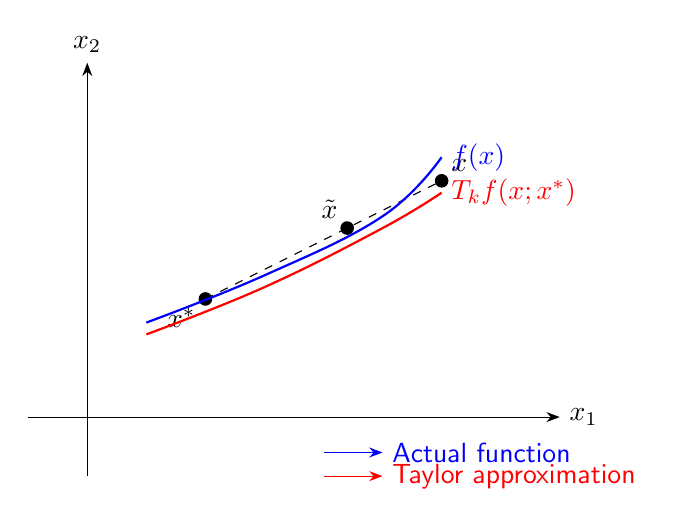
\begin{tikzpicture}[scale=1.5, >=Stealth]
    % Coordinate axes
    \draw[->] (-0.5,0) -- (4,0) node[right]{$x_1$};
    \draw[->] (0,-0.5) -- (0,3) node[above]{$x_2$};
    
    % Points
    \coordinate (xstar) at (1,1);
    \coordinate (x) at (3,2);
    \filldraw (xstar) circle (1.5pt) node[below left]{$x^*$};
    \filldraw (x) circle (1.5pt) node[above right]{$x$};
    
    % Line segment
    \draw[dashed] (xstar) -- (x);
    
    % Function surface
    \draw[blue, thick] plot[smooth, tension=0.7] coordinates {(0.5,0.8) (1.5,1.2) (2.5,1.7) (3,2.2)};
    \node[blue, right] at (3,2.2) {$f(x)$};
    
    % Taylor approximation
    \draw[red, thick] plot[smooth, tension=0.7] coordinates {(0.5,0.7) (1.5,1.1) (2.5,1.6) (3,1.9)};
    \node[red, right] at (3,1.9) {$T_k f(x; x^*)$};
    
    % Intermediate point
    \coordinate (xtilde) at ($(xstar)!0.6!(x)$);
    \filldraw[black] (xtilde) circle (1.5pt) node[above left]{$\tilde{x}$};
    
    % Legend
    \draw[->, blue] (2,-0.3) -- (2.5,-0.3) node[right]{Actual function};
    \draw[->, red] (2,-0.5) -- (2.5,-0.5) node[right]{Taylor approximation};
\end{tikzpicture}
\caption{Visualization of Taylor's theorem in \(\mathbb{R}^2\). The blue curve represents the actual function \( f \), while the red curve shows its \( k \)-th order Taylor approximation \( T_k f \) at \( x^* \). The point \( \tilde{x} \) lies on the line segment between \( x^* \) and \( x \).}
\end{figure}
\newpage 
\textbf{Problem} \\
Compute the Taylor polynomial of order 3 at \( x_0 = (1,0)^T \) for the function 
\[ f(x_1,x_2) = e^{x_1+x_2} + e^{x_1-x_2}. \]

\textbf{Solution}\\

We compute the gradient, the Hessian, and the partial derivatives of third order, evaluating them at the point \( x_0 \):

\subsubsection*{First Derivatives (Gradient)}
\[ \nabla f(x) = 
\begin{pmatrix}
e^{x_1+x_2} + e^{x_1-x_2} \\
e^{x_1+x_2} - e^{x_1-x_2}
\end{pmatrix}
\]
At \( x_0 = (1,0) \):
\[ \nabla f(1,0) = 
\begin{pmatrix}
e + 1 \\
e - 1
\end{pmatrix}
\]

\subsubsection*{Second Derivatives (Hessian)}
\[ H_f(x) = 
\begin{pmatrix}
e^{x_1+x_2} + e^{x_1-x_2} & e^{x_1+x_2} - e^{x_1-x_2} \\
e^{x_1+x_2} - e^{x_1-x_2} & e^{x_1+x_2} + e^{x_1-x_2}
\end{pmatrix}
\]
At \( x_0 = (1,0) \):
\[ H_f(1,0) = 
\begin{pmatrix}
e + 1 & e - 1 \\
e - 1 & e + 1
\end{pmatrix}
\]

\subsubsection*{Third Derivatives}
\begin{align*}
\frac{\partial^3 f}{\partial x_1^3}(x) &= e^{x_1+x_2} + e^{x_1-x_2} \\
\frac{\partial^3 f}{\partial x_1^2 \partial x_2}(x) &= e^{x_1+x_2} - e^{x_1-x_2} \\
\frac{\partial^3 f}{\partial x_1 \partial x_2^2}(x) &= e^{x_1+x_2} + e^{x_1-x_2} \\
\frac{\partial^3 f}{\partial x_2^3}(x) &= e^{x_1+x_2} - e^{x_1-x_2}
\end{align*}
At \( x_0 = (1,0) \):
\begin{align*}
\frac{\partial^3 f}{\partial x_1^3}(1,0) &= e + 1 \\
\frac{\partial^3 f}{\partial x_1^2 \partial x_2}(1,0) &= e - 1 \\
\frac{\partial^3 f}{\partial x_1 \partial x_2^2}(1,0) &= e + 1 \\
\frac{\partial^3 f}{\partial x_2^3}(1,0) &= e - 1
\end{align*}

\subsubsection*{Taylor Polynomial of Order 3}
The Taylor polynomial is given by:
\begin{align*}
T_3f(x; x_0) &= f(1,0) + \nabla f(1,0)^T \begin{pmatrix} x_1-1 \\ x_2 \end{pmatrix} + \frac{1}{2} \begin{pmatrix} x_1-1 & x_2 \end{pmatrix} H_f(1,0) \begin{pmatrix} x_1-1 \\ x_2 \end{pmatrix} \\
&\quad + \frac{1}{6} \left[ \frac{\partial^3 f}{\partial x_1^3}(1,0)(x_1-1)^3 + 3\frac{\partial^3 f}{\partial x_1^2 \partial x_2}(1,0)(x_1-1)^2x_2 \right. \\
&\quad \left. + 3\frac{\partial^3 f}{\partial x_1 \partial x_2^2}(1,0)(x_1-1)x_2^2 + \frac{\partial^3 f}{\partial x_2^3}(1,0)x_2^3 \right]
\end{align*}

Substituting the computed values:
\begin{align*}
T_3f(x; x_0) &= (e + 1) + [e(x_1-1) + (e-1)x_2] \\
&\quad + \frac{1}{2} \left[ (e+1)(x_1-1)^2 + 2(e-1)(x_1-1)x_2 + (e+1)x_2^2 \right] \\
&\quad + \frac{1}{6} \left[ (e+1)(x_1-1)^3 + 3(e-1)(x_1-1)^2x_2 + 3(e+1)(x_1-1)x_2^2 + (e-1)x_2^3 \right]
\end{align*}
\vspace{2mm}
\textbf{Problem} \\
Let \( f: \mathbb{R}^{2} \to \mathbb{R} \) be the function 
\[ f(x_{1}, x_{2}) = e^{x_{1}^{2} \cdot x_{2}} + \cos(\pi \cdot x_{1} \cdot x_{2}). \]

Determine a tangential plane to the graph of \( f \) at the point \( (1, -1)^{\top} \) in the form 
\[ \alpha_{1}x_{1} + \alpha_{2}x_{2} + \alpha_{3}x_{3} = \beta. \]

\textbf{Solution} \\

To find the tangential plane, we compute the first-order Taylor approximation (linear approximation) of \( f \) at \( (1, -1)^{\top} \).

\textbf{1. Compute the Gradient}
The gradient of \( f \) is:
\[ \nabla f(x_{1}, x_{2}) = 
\begin{pmatrix}
2x_{1}x_{2}e^{x_{1}^{2}x_{2}} - \pi x_{2} \sin(\pi x_{1}x_{2}) \\
x_{1}^{2}e^{x_{1}^{2}x_{2}} - \pi x_{1} \sin(\pi x_{1}x_{2})
\end{pmatrix}. \]

\textbf{2. Evaluate at \( (1, -1)^{\top} \)}
\[ f(1, -1) = e^{-1} + \cos(-\pi) = e^{-1} - 1, \]
\[ \nabla f(1, -1) = 
\begin{pmatrix}
-2e^{-1} + \pi \sin(-\pi) \\
e^{-1} - \pi \sin(-\pi)
\end{pmatrix} = 
\begin{pmatrix}
-2e^{-1} \\
e^{-1}
\end{pmatrix}. \]

\textbf{3. Construct the Tangential Plane}\\
The equation of the tangential plane is:
\[ x_{3} = f(1, -1) + \nabla f(1, -1)^{\top} \cdot \begin{pmatrix} x_{1} - 1 \\ x_{2} + 1 \end{pmatrix}, \]
which simplifies to:
\[ x_{3} = e^{-1} - 1 - 2e^{-1}(x_{1} - 1) + e^{-1}(x_{2} + 1). \]

Rearranging terms:
\[ x_{3} = e^{-1} - 1 + 2e^{-1} + e^{-1} - 2e^{-1}x_{1} + e^{-1}x_{2}, \]
\[ 2e^{-1}x_{1} - e^{-1}x_{2} + x_{3} = 4e^{-1} - 1. \]

\textbf{4. Final Form} \\
The coefficients are:
\[ \alpha_{1} = 2e^{-1}, \quad \alpha_{2} = -e^{-1}, \quad \alpha_{3} = 1, \quad \beta = 4e^{-1} - 1. \]

Thus, the tangential plane equation is:
\[ 2e^{-1}x_{1} - e^{-1}x_{2} + x_{3} = 4e^{-1} - 1. \]
\newpage
\section{Local Optima of Multivariate Functions}

\subsubsection*{Definition}
Let \( X \subseteq \mathbb{R}^n \) be open, \( f: X \to \mathbb{R} \).

\begin{enumerate}
    \item[(1)] A point \( x^* \in X \) is called a \textit{(strict) local minimum} of \( f \) if there is a \(\delta\)-neighborhood \( N_\delta(x^*) \) of \( x^* \) such that 
    \[ f(x^*) \leq f(x), \quad \text{for all } x \in X \cap N_\delta(x^*). \]

    \item[(2)] A point \( x^* \in X \) is called a \textit{(strict) local maximum} of \( f \) if there is a \(\delta\)-neighborhood \( N_\delta(x^*) \) of \( x^* \) such that
    \[ f(x^*) \geq f(x), \quad \text{for all } x \in X \cap N_\delta(x^*). \]

    \item[(3)] A point \( x^* \) is called a \textit{(strict) global maximizer/minimizer} of \( f \) if 
    \[ f(x^*) \geq f(x) \text{ for all } x \in X \]
    or
    \[ f(x^*) \leq f(x) \text{ for all } x \in X, \]
    respectively.

    \item[(4)] The respective function values are called \textit{(strict) local/global minimum/maximum} of \( f \).

    \item[(5)] A local/global minimum or maximum is also referred to as an \textit{extremum} or \textit{optimum} of \( f \).
\end{enumerate}

\subsection{Optimality Condition}
If \( x^* \) is a local minimizer and \( x^* \) is an interior point, then it can be analyzed as follows:

Let 
\[ x := x^* - \epsilon \nabla f(x^*), \]
while 
\[ f(x) = f(x^*) + \nabla f(x^*)^T (x - x^*) + r(x - x^*). \]

Substituting \( x \):
\[ f(x) = f(x^*) + Df(x^*)^T (-\varepsilon \nabla f(x^*)) + r(x - x^*) \]
\[ = f(x^*) - \epsilon \| \nabla f(x^*) \|^2 + r(x - x^*). \]

As \( r(x - x^*) \to 0 \) when \( x \to x^* \), this implies that for sufficiently small \( \epsilon \), the term \( -\epsilon \| \nabla f(x^*) \|^2 \) dominates, leading to:
\[ f(x) < f(x^*), \]
unless \( \nabla f(x^*) = 0 \). 

\subsubsection*{Theorem}
Let \( X \subseteq \mathbb{R}^n \) be open, \( x^* \in X \), and \( f: X \to \mathbb{R} \) differentiable at \( x^* \). If \( x^* \) is a local optimum of \( f \), then 
\[ \nabla f(x^*) = 0. \]
This is a necessary, but not sufficient, condition for optimality.

\subsubsection*{Definition}
Let \( X \subseteq \mathbb{R}^n \) be open, \( f: X \to \mathbb{R} \) differentiable.

\begin{enumerate}
    \item[(1)] A point \( x^* \in X \) with \( \nabla f(x^*) = 0 \) is called a \textit{stationary point} of \( f \).

    \item[(2)] If \( x^* \in X \) is a stationary point but not a local extremum, it is called a \textit{saddle point}.
\end{enumerate}
\subsection{Local Optima of Multivariate Functions}
\subsubsection*{Problem Setup}
Assume \( f \in e^2(X) \) for \( X \subseteq \mathbb{R}^n \) and \( x^* \in X \) with \( Df(x^*) = 0 \). How can we determine whether \( x^* \) is a local minimum, local maximum, or a saddle point?

\subsubsection{Taylor Expansion Approach}
Using the second-order Taylor expansion around \( x^* \):
\[
f(x) = f(x^*) + Df(x^*)^T (x - x^*) + \frac{1}{2} (x - x^*)^T H_f(x^*) (x - x^*) + \cdots,
\]
where \( H_f(x^*) \) is the Hessian matrix of \( f \) at \( x^* \). Since \( Df(x^*) = 0 \), the local behavior of \( f \) at \( x^* \) is governed by the quadratic form:
\[
(x - x^*)^T H_f(x^*) (x - x^*).
\]

\subsubsection{Definition of Definite Matrices}
Let \( A \in \mathbb{R}^{n \times n} \) be symmetric. Then \( A \) is called:
\begin{enumerate}
    \item \textit{positive definite} if \( v^T A v > 0 \) for all \( v \in \mathbb{R}^n \setminus \{0\} \);
    \item \textit{positive semidefinite} if \( v^T A v \geq 0 \) for all \( v \in \mathbb{R}^n \setminus \{0\} \);
    \item\textit{negative definite} if \( v^T A v < 0 \) for all \( v \in \mathbb{R}^n \setminus \{0\} \);
    \item \textit{negative semidefinite} if \( v^T A v \leq 0 \) for all \( v \in \mathbb{R}^n \setminus \{0\} \);
    \item \textit{indefinite} if there exist \( v, w \in \mathbb{R}^n \setminus \{0\} \) such that \( v^T A v > 0 \) and \( w^T A w < 0 \).
\end{enumerate}

\subsection*{Remark}
A matrix \( A \) is negative definite if and only if \( -A \) is positive definite.

\subsection*{Theorem: Classification of Stationary Points}
Let \( X \subseteq \mathbb{R}^n \) be open, \( f \in C^2(X) \), and \( x^* \in X \) a stationary point (i.e., \( Df(x^*) = 0 \)). Then:
\begin{enumerate}
    \item If \( x^* \) is a local minimizer of \( f \), then \( H_f(x^*) \) is positive semidefinite.
    \item If \( H_f(x^*) \) is positive definite, then \( x^* \) is a local minimizer of \( f \).
    \item If \( x^* \) is a local maximizer of \( f \), then \( H_f(x^*) \) is negative semidefinite.
    \item If \( H_f(x^*) \) is negative definite, then \( x^* \) is a local maximizer of \( f \).
    \item If \( H_f(x^*) \) is indefinite, then \( x^* \) is a saddle point.
\end{enumerate}
\subsection*{Example (a)}
Consider \( f : \mathbb{R}^2 \rightarrow \mathbb{R} \) defined by:
\[
f(x_1, x_2) = 2 - (x_1 - 1)^2 - (x_2 - 1)^2.
\]

\subsubsection*{Finding Stationary Points}
The gradient is:
\[
\nabla f(x) = 
\begin{pmatrix}
-2(x_1 - 1) \\
-2(x_2 - 1)
\end{pmatrix}
=
\begin{pmatrix}
0 \\
0
\end{pmatrix}
\implies
\begin{cases}
x_1 = 1, \\
x_2 = 1.
\end{cases}
\]
Thus, the stationary point is \( x^* = \begin{pmatrix} 1 \\ 1 \end{pmatrix} \).

\subsubsection*{Classification}
The Hessian matrix is:
\[
H_f(x) = 
\begin{pmatrix}
-2 & 0 \\
0 & -2
\end{pmatrix}.
\]
For any \( v = \begin{pmatrix} v_1 \\ v_2 \end{pmatrix} \neq 0 \):
\[
v^T H_f(1,1) v = -2v_1^2 - 2v_2^2 < 0.
\]
Since the Hessian is \textit{negative definite}, \( x^* \) is a \textit{local maximum}.

\subsection*{Example (b)}
Consider \( f : \mathbb{R}^2 \rightarrow \mathbb{R} \) defined by:
\[
f(x_1, x_2) = 7 - x_1^2 - x_2^2 + 3x_1 x_2.
\]

\subsubsection*{Finding Stationary Points}
The gradient is:
\[
\nabla f(x) = 
\begin{pmatrix}
-2x_1 + 3x_2 \\
-2x_2 + 3x_1
\end{pmatrix}
=
\begin{pmatrix}
0 \\
0
\end{pmatrix}.
\]
Solving the system:
\[
\begin{cases}
-2x_1 + 3x_2 = 0, \\
3x_1 - 2x_2 = 0,
\end{cases}
\]
we find \( x^* = \begin{pmatrix} 0 \\ 0 \end{pmatrix} \).

\subsubsection*{Classification}
The Hessian matrix is:
\[
H_f(x) = 
\begin{pmatrix}
-2 & 3 \\
3 & -2
\end{pmatrix}.
\]
For \( v = \begin{pmatrix} 1 \\ 0 \end{pmatrix} \):
\[
v^T H_f(0,0) v = -2 < 0.
\]
For \( v = \begin{pmatrix} 1 \\ 1 \end{pmatrix} \):
\[
v^T H_f(0,0) v = -2 - 2 + 6 = 2 > 0.
\]
Since the Hessian is \textit{indefinite}, \( x^* \) is a \textit{saddle point}.

\subsection*{Example (c)}
Consider \( f : \mathbb{R}^2 \rightarrow \mathbb{R} \) defined by:
\[
f(x_1, x_2) = x_1 x_2.
\]

\subsubsection*{Finding Stationary Points}
The gradient is:
\[
\nabla f(x) = 
\begin{pmatrix}
x_2 \\
x_1
\end{pmatrix}
=
\begin{pmatrix}
0 \\
0
\end{pmatrix}
\implies x^* = \begin{pmatrix} 0 \\ 0 \end{pmatrix}.
\]

\subsubsection*{Classification}
The Hessian matrix is:
\[
H_f(x) = 
\begin{pmatrix}
0 & 1 \\
1 & 0
\end{pmatrix}.
\]
For \( v = \begin{pmatrix} 1 \\ 1 \end{pmatrix} \):
\[
v^T H_f(0,0) v = 2 > 0.
\]
For \( v = \begin{pmatrix} 1 \\ -1 \end{pmatrix} \):
\[
v^T H_f(0,0) v = -2 < 0.
\]
Since the Hessian is \textit{indefinite}, \( x^* \) is a \textit{saddle point}.
\section*{Sylvester's Determinant Criterion for Definiteness}

\subsection*{Theorem (Sylvester's Criterion)}
For a symmetric matrix \( A \in \mathbb{R}^{n \times n} \), \( A = [a_{ij}]_{i,j=1}^n \), define the leading principal submatrices:
\[
A_k := [a_{ij}]_{i,j=1}^k \quad \text{for} \quad k = 1, \dots, n.
\]

\begin{enumerate}
    \item[(1)] \( A \) is \textit{positive definite} if and only if all leading principal minors \( \det(A_k) > 0 \) for \( k = 1, \dots, n \).

    \item[(2)] \( A \) is \textit{negative definite} if and only if:
    \begin{itemize}
        \item \( \det(A_k) < 0 \) for all odd \( k \),
        \item \( \det(A_k) > 0 \) for all even \( k \).
    \end{itemize}
\end{enumerate}

\subsection*{Remark}
\( A \) is negative definite if and only if \( -A \) is positive definite. This implies:
\[
\det(-A_k) = (-1)^k \det(A_k) > 0 \quad \text{for all} \quad k.
\]

\section*{Examples}

\subsection*{Example (a)}
Consider the matrix:
\[
A = \begin{pmatrix}
2 & 0 \\
0 & 2
\end{pmatrix}.
\]
\begin{itemize}
    \item \( \det(A_1) = \det(2) = 2 > 0 \),
    \item \( \det(A_2) = \det \begin{pmatrix} 2 & 0 \\ 0 & 2 \end{pmatrix} = 4 > 0 \).
\end{itemize}
Since all leading principal minors are positive, \( A \) is \textit{positive definite}.

\subsection*{Example (b)}
Consider the matrix:
\[
A = \begin{pmatrix}
-2 & 3 \\
3 & -2
\end{pmatrix}.
\]
\begin{itemize}
    \item \( \det(A_1) = \det(-2) = -2 < 0 \),
    \item \( \det(A_2) = \det \begin{pmatrix} -2 & 3 \\ 3 & -2 \end{pmatrix} = 4 - 9 = -5 < 0 \).
\end{itemize}
Since \( \det(A_1) < 0 \) (odd \( k \)) but \( \det(A_2) < 0 \) (even \( k \)), the conditions for negative definiteness are \textit{not} satisfied. Instead, \( A \) is \textit{indefinite}.

\subsection*{Example (c)}
Consider the matrix:
\[
A = \begin{pmatrix}
2 & -1 & -1 \\
-1 & 2 & 1 \\
-1 & 1 & 1
\end{pmatrix}.
\]
\begin{itemize}
    \item \( \det(A_1) = \det(2) = 2 > 0 \),
    \item \( \det(A_2) = \det \begin{pmatrix} 2 & -1 \\ -1 & 2 \end{pmatrix} = 4 - 1 = 3 > 0 \),
    \item \( \det(A_3) = \det \begin{pmatrix} 2 & -1 & -1 \\ -1 & 2 & 1 \\ -1 & 1 & 1 \end{pmatrix} \).

    To compute \( \det(A_3) \):
    \[
    \det(A_3) = 2 \cdot \det \begin{pmatrix} 2 & 1 \\ 1 & 1 \end{pmatrix} - (-1) \cdot \det \begin{pmatrix} -1 & 1 \\ -1 & 1 \end{pmatrix} + (-1) \cdot \det \begin{pmatrix} -1 & 2 \\ -1 & 1 \end{pmatrix}
    \]
    \[
    = 2(2 \cdot 1 - 1 \cdot 1) + 1(-1 \cdot 1 - 1 \cdot (-1)) - 1(-1 \cdot 1 - 2 \cdot (-1))
    \]
    \[
    = 2(1) + 1(0) - 1(1) = 2 + 0 - 1 = 1 > 0.
    \]
\end{itemize}
Since all leading principal minors are positive, \( A \) is \textit{positive definite}.
\vspace{10mm}
\section{Numerical Optimization Methods}
determining stationary points of functions may be very difficult or maybe not even possible - think of a function implicitly defined as the solution of a convoluted differential equation system. Hence, in practice numerical methods that approximate an optimal solution are used frequently
\subsection*{Interpretation of the Gradient}
Consider \( f: X \rightarrow \mathbb{R} \) differentiable at \( x^* \in X \). For a direction \( v \in \mathbb{R}^n \setminus \{0\} \) with \( \|v\| = 1 \), the directional derivative \( \partial_v f(x^*) \) represents the local rate of change of \( f \) at \( x^* \) in direction \( v \). It satisfies:

\[
|\partial_v f(x^*)| = |(\nabla f(x^*))^T v| \leq \|\nabla f(x^*)\| \cdot \|v\| = \|\nabla f(x^*)\|
\]

\subsection*{Steepest Ascent/Descent Directions}
The norm of the gradient \( \|\nabla f(x^*)\| \) measures the maximum local rate of change of \( f \) at \( x^* \). 

For the normalized direction:
\[
v = \frac{\nabla f(x^*)}{\|\nabla f(x^*)\|}
\]
we obtain the maximal directional derivative:
\[
\partial_v f(x^*) = \nabla f(x^*)^T \cdot \frac{\nabla f(x^*)}{\|\nabla f(x^*)\|} = \|\nabla f(x^*)\|
\]

\begin{itemize}
    \item \( \nabla f(x^*) \) points in the direction of \textit{steepest ascent}
    \item \( -\nabla f(x^*) \) points in the direction of \textit{steepest descent}
\end{itemize}

\subsection*{Definition}
Let \( X \subseteq \mathbb{R}^n \) be open, \( f \in C^1(X) \), and \( x^* \in X \) with \( \nabla f(x^*) \neq 0 \). The normalized vectors:
\[
\frac{\nabla f(x^*)}{\|\nabla f(x^*)\|} \quad \text{(steepest ascent)}, \quad -\frac{\nabla f(x^*)}{\|\nabla f(x^*)\|} \quad \text{(steepest descent)}
\]
give the directions of maximal increase/decrease of \( f \) at \( x^* \).

\subsection*{Geometric Interpretation}
\begin{center}
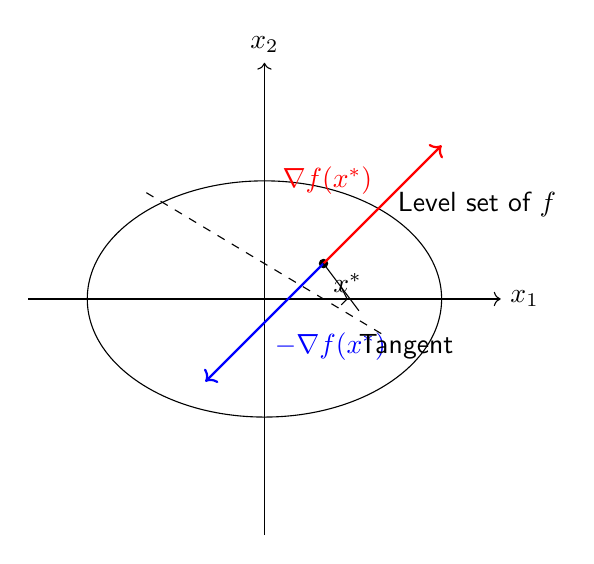
\begin{tikzpicture}[scale=1.5]
    % Axes
    \draw[->] (-2,0) -- (2,0) node[right]{$x_1$};
    \draw[->] (0,-2) -- (0,2) node[above]{$x_2$};
    
    % Level curve (ellipse)
    \draw (0,0) ellipse (1.5 and 1);
    \node at (1.8,0.8) {Level set of $f$};
    
    % Point x*
    \filldraw (0.5,0.3) circle (1pt) node[below right]{$x^*$};
    
    % Gradient vectors
    \draw[->, thick, red] (0.5,0.3) -- (1.5,1.3) node[midway, above left]{$\nabla f(x^*)$};
    \draw[->, thick, blue] (0.5,0.3) -- (-0.5,-0.7) node[midway, below right]{$-\nabla f(x^*)$};
    
    % Tangent line
    \draw[dashed] (-1,0.9) -- (1,-0.3);
    \node at (1.2,-0.4) {Tangent};
    
    % Orthogonality indication
    \draw (0.5,0.3) -- (0.8,-0.1);
    \draw (0.65,0.1) -- (0.7,0.0) -- (0.65,-0.05);
\end{tikzpicture}
\end{center}

Key observations:
\begin{itemize}
    \item The gradient \( \nabla f(x^*) \) is orthogonal to the tangent of the level set at \( x^* \)
    \item It points in the direction of greatest increase of \( f \)
    \item The negative gradient points in the direction of greatest decrease
\end{itemize}
\subsection{Algorithm for Gradient Descent Method}
\begin{enumerate}
    \item \textbf{Initialize:}
    \begin{itemize}
    \item Set $k := 0$ (iteration counter)
    \end{itemize}
    
    \item \textbf{While} $\nabla f(x^{(k)}) \neq 0$ \textbf{or} $\|Df(x^{(k)})\| > \epsilon$:
    \begin{itemize}
    \item Set search direction: $v := \dfrac{-Df(x^{(k)})}{\|Df(x^{(k)})\|}$
    \item Find step size $\lambda \in [0, \infty)$ such that:
    \[ f(x^{(k)} + \lambda v) < f(x^{(k)}) \]
    \item Update: $x^{(k+1)} := x^{(k)} + \lambda v$
    \item Increment: $k := k + 1$
    \end{itemize}
    
    \item \textbf{End While}
    \end{enumerate}
    
    \subsubsection*{Step Size Selection Methods}
    
    \begin{itemize}
    \item \textbf{Line Search:}
    \begin{itemize}
    \item Determine $\lambda$ that minimizes $f(x^{(k)} + \lambda v)$
    \end{itemize}
    
    \item \textbf{Heuristic Approach:}
    \begin{itemize}
    \item Start with $\lambda := 1$
    \item If $f(x^{(k)} + \lambda v) \geq f(x^{(k)})$:
    \begin{itemize}
    \item Set $\lambda := \frac{1}{2}\lambda$
    \item Repeat until $f(x^{(k)} + \lambda v) < f(x^{(k)})$
    \item Keep final $\lambda$ for next step
    \end{itemize}
    \item Else:
    \begin{itemize}
    \item Try $\tilde{\lambda} := 2\lambda$
    \item If $f(x^{(k)} + \tilde{\lambda}v) < f(x^{(k)})$:
    \begin{itemize}
    \item Use $\tilde{\lambda}$ as new step size
    \end{itemize}
    \item Else keep original $\lambda$
    \end{itemize}
    \end{itemize}
    \end{itemize}
    
    \subsubsection*{Algorithm Specification}
    
    \textbf{Input:}
    \begin{itemize}
    \item $f \in C^1(\mathbb{R}^n)$ (continuously differentiable function)
    \item Initial value $x \in \mathbb{R}^n$
    \end{itemize}
    
    \textbf{Output:}
    \begin{itemize}
    \item Point $x^* \in \mathbb{R}^n$ approximating a local minimum of $f$
    \end{itemize}

    \vspace{5mm}
    Gradient descent uses a linear approximation of function $f$. Can we use a quadratic approximation instead?
    
    \[ T_2 f(x; x^{(k)}) = f(x^{(k)}) + Df(x^{(k)})^T (x - x^{(k)}) + \frac{1}{2} (x - x^{(k)})^T H_f(x^{(k)}) (x - x^{(k)}) \]
    
    Find a stationary point/minimum of $T_2 f(x; x^{(k)})$:
    
    \[ 0 = \nabla T_2 f(x; x^{(k)}) = \nabla f(x^{(k)}) + H_f(x^{(k)}) (x - x^{(k)}) \]
    \[ \Leftrightarrow H_f(x^{(k)}) (x - x^{(k)}) = -\nabla f(x^{(k)}) \]
    
    \[
    \underbrace{\text{This is Newton's equation}}_{\text{Update rule: } x^{(k+1)} = x^{(k)} + (x - x^{(k)})}
    \]
    
    Works well if $H_f(x^{(k)})$ is positive definite $\rightarrow$ local minimum approximation.
    
    \subsection*{Algorithm: Newton's Method}
    
    \textbf{Input:}
    \begin{itemize}
    \item $f \in C^2(\mathbb{R}^n)$ (twice differentiable)
    \item Initial value $x \in \mathbb{R}^n$
    \end{itemize}
    
    \textbf{Output:}
    \begin{itemize}
    \item $x^*$ approximating a local minimizer of $f$
    \item Or indication that Newton's equation cannot be solved
    \end{itemize}
    
    \begin{enumerate}
    \item Initialize $k := 0$
    \item While $\|Df(x^{(k)})\| \neq 0$ (or $\|Df(x^{(k)})\| \geq \epsilon$):
    \begin{itemize}
    \item Find $v \in \mathbb{R}^n$ that solves:
    \[ H_f(x^{(k)}) v = -Df(x^{(k)}) \]
    \item If no solution exists: terminate with error
    \item Update:
    \[ x^{(k+1)} := x^{(k)} + v \]
    (Alternative: $x^{(k+1)} := x^{(k)} + \alpha v$ for some step size $\alpha$)
    \item Increment: $k := k + 1$
    \end{itemize}
    \item Return $x^* := x^{(k)}$
    \end{enumerate}
\vspace{5mm}
\section{Constrained Optimization \& the KKT theorem}
\subsection*{Problem Setting}
\begin{align*}
\min\ & f(x) \\
\text{s.t.}\ & h(x) = 0
\end{align*}
where:
\begin{itemize}
    \item $f: \mathbb{R}^n \rightarrow \mathbb{R}$ is the objective function
    \item $h: \mathbb{R}^n \rightarrow \mathbb{R}^m$ defines constraints
\end{itemize}

\subsection*{Definitions}
\begin{itemize}
    \item \textbf{Feasible set:} $F := \{ x \in \mathbb{R}^n : h(x) = 0 \}$
    \item \textbf{Lagrange function:} For $z \in \mathbb{R}^m$,
    \[ L(x,z) := f(x) + h(x)^T z \]
\end{itemize}

\subsection{Theorem (Lagrange Multipliers)}
Let $X \subseteq \mathbb{R}^n$ be open, $f: X \rightarrow \mathbb{R}$ and $h: X \rightarrow \mathbb{R}^k$ be continuously differentiable. Consider:
\begin{align*}
\min_x\ & f(x) \\
\text{s.t.}\ & h(x) = 0
\end{align*}
If $x^* \in F$ is an extremum point of $f$ over $F$ and $\text{rank}(Jh(x^*)) = \min\{n,m\}$, then there exist Lagrange multipliers $z^* \in \mathbb{R}^k$ such that:
\[ Df(x^*) + Jh(x^*)^T z^* = 0 \]
\[ \Rightarrow Df(x^*) + \sum_{i=1}^k Dh_i(x^*) \zeta_i^* = 0 \]
\subsection{KKT Conditions for Constrained Optimization}

\subsection*{General Problem Setting}
\begin{align*}
\min\ & f(x) \\
\text{s.t.}\ & g(x) \leq 0 \\
& h(x) = 0
\end{align*}
where:
\begin{itemize}
\item $f: \mathbb{R}^n \rightarrow \mathbb{R}$ is the objective function
\item $g: \mathbb{R}^n \rightarrow \mathbb{R}^m$ defines inequality constraints
\item $h: \mathbb{R}^n \rightarrow \mathbb{R}^\ell$ defines equality constraints
\end{itemize}

\subsubsection*{Definition (KKT Point)}
Let $X \subseteq \mathbb{R}^n$ be open, with $f:X\rightarrow\mathbb{R}$, $g:X\rightarrow\mathbb{R}^m$, and $h:X\rightarrow\mathbb{R}^\ell$ all continuously differentiable. A point $(x^*, y^*, z^*) \in X \times \mathbb{R}^m \times \mathbb{R}^\ell$ is called a \textbf{KKT point} (Karush-Kuhn-Tucker point) if:

\subsection*{KKT Conditions}
\begin{enumerate}[label=(\arabic*)]
    \item \textbf{Stationarity}:
    \[ \nabla f(x^*) + \sum_{i=1}^m y_i^* \nabla g_i(x^*) + \sum_{j=1}^\ell z_j^* \nabla h_j(x^*) = 0 \]
    
    \item \textbf{Primal feasibility}:
    \[ g(x^*) \leq 0 \quad \text{and} \quad h(x^*) = 0 \]
    
    \item \textbf{Dual feasibility}:
    \[ y^* \geq 0 \]
    
    \item \textbf{Complementary slackness}:
    \[ (y^*)^T g(x^*) = 0 \quad \Leftrightarrow \quad y_i^* \cdot g_i(x^*) = 0 \ \forall i \in \{1,\ldots,m\} \]
\end{enumerate}

\subsection{Theorem (Necessary Optimality Conditions)}
Let $X \subseteq \mathbb{R}^n$ be open, with $f:X\rightarrow\mathbb{R}$, $g:X\rightarrow\mathbb{R}^m$, and $h:X\rightarrow\mathbb{R}^\ell$ continuously differentiable. If $x^* \in X$ is a local minimizer and the \textbf{constraint qualification} holds:
\[
\{ \nabla g_i(x^*) : g_i(x^*) = 0 \} \cup \{ \nabla h_j(x^*) \} \text{ are linearly independent}
\]
then there exist $y^* \in \mathbb{R}^m$, $z^* \in \mathbb{R}^\ell$ such that $(x^*, y^*, z^*)$ is a KKT point.
\vspace{5mm}
\subsection*{Problem}
The constraint $x\in C$ may be expressed as
\[
\left\|\begin{pmatrix}x_{1}\\ x_{2}\end{pmatrix}-\begin{pmatrix}1\\ 0\end{pmatrix}\right\|^{2}=9
\]
\[
\Leftrightarrow (x_{1}-1)^{2}+x_{2}^{2}-9=0
\]

The optimization problem to solve is therefore given by
\[
\min f(x_{1},x_{2})=2x_{1}+x_{2}
\]
subject to $\hspace{7.227pt}h(x_{1},x_{2})=(x_{1}-1)^{2}+x_{2}^{2}-9=0$.

Let us first state that the objective is a continuous function and the feasible set is clearly compact, so we can be sure that a minimizer of $f$ over the circle actually exists.

The objective function is convex, so we can try to apply the method of Lagrange multipliers. To do that, we first need the differentials of $f$ and $h$:
\[
\nabla f(x_{1},x_{2})=\begin{pmatrix}2\\ 1\end{pmatrix}
\]
\[
J_{h}(x_{1},x_{2})=\begin{pmatrix}2(x_{1}-1)\\ 2x_{2}\end{pmatrix}^{\top}
\]

With Lagrange multiplier $\zeta\in\mathbb{R}$, we get the following condition for a minimizer $x^{*}$:
\[
\nabla f(x)+J_{h}(x)^{\top}\cdot\zeta=0
\]
\[
\Leftrightarrow \begin{pmatrix}2+2\zeta(x_{1}-1)\\ 1+2\zeta x_{2}\end{pmatrix}=\begin{pmatrix}0\\ 0\end{pmatrix}
\]

Together with the condition $x\in C$ we get the following nonlinear equation system:
\[
2\zeta x_{1}=-2+2\zeta
\]
\[
2\zeta x_{2}=-1
\]
\[
(x_{1}-1)^{2}+x_{2}^{2}=9
\]

Let us first investigate the case $\zeta\neq 0$. We can then solve the first two equations for $x_{1}$ and $x_{2}$, respectively:
\[
x_{1}=\frac{-1+\zeta}{\zeta}\quad\text{for }\zeta\neq 0
\]
\[
x_{2}=\frac{-1}{2\zeta}\quad\text{for }\zeta\neq 0
\]

Substituting these into the third equation yields
\[
\left(\frac{-1+\zeta}{\zeta}-1\right)^{2}+\left(\frac{-1}{2\zeta}\right)^{2}=9
\]
\[
\Leftrightarrow \left(\frac{-1}{\zeta}\right)^{2}+\left(\frac{-1}{2\zeta}\right)^{2}=9
\]
\[
\Leftrightarrow \frac{1}{\zeta^{2}}+\frac{1}{4\zeta^{2}}=9
\]
\[
\Leftrightarrow \frac{5}{4\zeta^{2}}=9
\]
\[
\Leftrightarrow \frac{5}{36}=\zeta^{2}
\]

This in turn yields the following candidates for a minimizer:
\[
x^{*} =\begin{pmatrix}\frac{-1+\zeta}{\zeta}\\ \frac{-1}{2\zeta}\end{pmatrix}=\begin{pmatrix}\frac{-1}{\zeta}+1\\ \frac{-1}{2\zeta}\end{pmatrix}=\begin{pmatrix}\frac{-6}{\sqrt{5}}+1\\ \frac{-1}{2\cdot\frac{\sqrt{5}}{6}}\end{pmatrix}=\begin{pmatrix}\frac{-6+\sqrt{5}}{\sqrt{5}}\\ \frac{-3}{\sqrt{5}}\end{pmatrix}=-\frac{1}{\sqrt{5}}\begin{pmatrix}6-\sqrt{5}\\ 3\end{pmatrix}
\]
\[
x^{**} =\begin{pmatrix}\frac{-1+\zeta}{\zeta}\\ \frac{-1}{2\zeta}\end{pmatrix}=\begin{pmatrix}\frac{-1}{\zeta}+1\\ \frac{-1}{2\zeta}\end{pmatrix}=\begin{pmatrix}\frac{6}{\sqrt{5}}+1\\ \frac{-1}{2\cdot\frac{-\sqrt{5}}{6}}\end{pmatrix}=\begin{pmatrix}\frac{6+\sqrt{5}}{\sqrt{5}}\\ \frac{3}{\sqrt{5}}\end{pmatrix}=\frac{1}{\sqrt{5}}\begin{pmatrix}6+\sqrt{5}\\ 3\end{pmatrix}
\]

A quick check verifies that both candidate points are contained in the feasible set $C$:
\[
\left\|x^{*}-\begin{pmatrix}1\\ 0\end{pmatrix}\right\|^{2} =\left\|\frac{1}{\sqrt{5}}\begin{pmatrix}6-\sqrt{5}+\sqrt{5}\\ 3\end{pmatrix}\right\|^{2}=\frac{1}{5}(36+9)=9=3^{2}
\]
\[
\left\|x^{**}-\begin{pmatrix}1\\ 0\end{pmatrix}\right\|^{2} =\left\|\frac{1}{\sqrt{5}}\begin{pmatrix}6+\sqrt{5}-\sqrt{5}\\ 3\end{pmatrix}\right\|^{2}=\frac{1}{5}(36+9)=9=3^{2}
\]

To find the minimizer of our objective function, we simply compare the objective values of $x^{*}$ and $x^{**}$:
\[
f(x^{*}) =\frac{-2\cdot(6-\sqrt{5})}{\sqrt{5}}+\frac{-3}{\sqrt{5}}=\frac{-15+2\sqrt{5}}{\sqrt{5}}
\]
\[
f(x^{**}) =\frac{2\cdot(6+\sqrt{5})}{\sqrt{5}}+\frac{3}{\sqrt{5}}=\frac{15+2\sqrt{5}}{\sqrt{5}}
\]

Clearly, the value for $x^{*}$ is lower, so this is the desired minimizer of $f$ over the circle $C$.

Remember, we still have to take care of the case $\zeta=0$ in our equation system
\[
2\zeta x_{1} =-2+2\zeta
\]
\[
2\zeta x_{2} =-1
\]
\[
(x_{1}-1)^{2}+x_{2}^{2} =9
\]

Substituting that value for $\zeta$ yields the system
\[
0 =-2
\]
\[
0 =-1
\]
\[
(x_{1}-1)^{2}+x_{2}^{2} =9
\]
That clearly is a contradiction, thus there is no solution of the equation system for $\zeta = 0$. The above
minimizer $x^{*}$ is therefore unique
\section{Convex Optimization}
\subsection{Convex Functions and Convex Sets}
\subsubsection*{Definitions}
\begin{itemize}
    \item[(1)] A set $X \subseteq \mathbb{R}^n$ is \textbf{convex} if $\forall x,y \in X$, the line segment between them is also contained in $X$:
    \[ \{\lambda x + (1-\lambda)y \mid \lambda \in [0,1]\} \subseteq X \]
    
    \begin{center}
    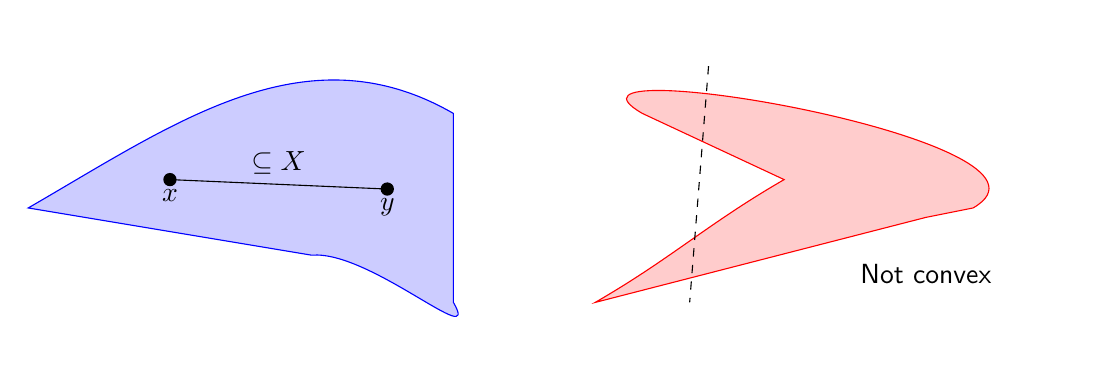
\begin{tikzpicture}[scale=1.2]
        % Convex set    
        \filldraw[fill=blue!20, draw=blue] (-1,0) to [out=30,in=150] (3.5,1) -- (3.5,-1) to [out=300,in=5] (2,-0.5) -- cycle;
        \draw (0.5,0.3) -- (2.8,0.2) node[midway,above] {$\subseteq X$};
        \fill (0.5,0.3) circle (2pt) node[below]{$x$};
        \fill (2.8,0.2) circle (2pt) node[below]{$y$};
        
        % Non-convex set
        \filldraw[fill=red!20, draw=red] (9,0) to [out=30,in=150] (5.5,1) -- (7,0.3) 
            to [out=210,in=30] (5,-1) -- (8.5,-0.1) -- cycle;
        \draw[dashed] (6.2,1.5) -- (6,-1);
        \node at (8.5,-0.7) {Not convex};
    \end{tikzpicture}
    \end{center}

    \item[(2)] For convex $X$, $f:X\to\mathbb{R}$ is \textbf{(strictly) convex} if $\forall x,y\in X$ and $\lambda\in(0,1)$:
    \[ f(\lambda x + (1-\lambda)y) \ (\textcolor{red}{<})\ \leq\ \lambda f(x) + (1-\lambda)f(y) \]
    
    \item[(3)] A function $f : X \rightarrow \mathbb{R}$ on a convex set $X \subseteq \mathbb{R}^{n}$ is called \textbf{concave} if $(-f)$ is convex

    \begin{center}
    \begin{tikzpicture}[scale=1.5]
        % Convex function
        \draw[->] (-0.5,0) -- (4,0);
        \draw[->] (0,-0.5) -- (0,3);
        \draw[blue, thick, domain=0.5:3.5, smooth] plot (\x, {0.3*(\x-2)^2 + 0.52});
        \draw[dashed] (0.8,0.63) -- (3.9,1.04);
        \fill (1.3,0.68) circle (1.7pt) node[below left]{$(x,f(x))$};
        \fill (3.2,0.95) circle (1.7pt) node[below right]{$(y,f(y))$};
        \node at (2,1.8) {Convex function};
        
        % Non-convex function
        \draw[->] (5,0) -- (9.5,0);
        \draw[->] (6,-0.5) -- (6,3);
        \draw[red, thick, domain=6.5:8.5, smooth] plot (\x, {-0.5*(\x-7.5)^2 + 2});
        \draw[dashed] (6.5,1.875) -- (8.5,1.875);
        \node at (7.5,0.5) {Non-convex};
    \end{tikzpicture}
    \end{center}
\end{itemize}

\subsection*{Theorem (Convexity and Hessian)}
Let $X \subseteq \mathbb{R}^n$ be open and convex, $f \in C^2(X)$.
\begin{itemize}
    \item[(1)] $f$ is convex $\Leftrightarrow H_f(x)$ is positive semidefinite $\forall x \in X$
    \item[(2)] If $H_f(x)$ is positive definite $\forall x \in X$, then $f$ is strictly convex
\end{itemize}

\subsection*{Examples}
\begin{itemize}
    \item \textbf{Convex:} $f(x) = x^2$, $f(x,y) = x^2 + y^2$
    \item \textbf{Strictly convex:} $f(x) = e^x$, $f(x,y) = x^2 + 2y^2$
    \item \textbf{Non-convex:} $f(x) = \sin x$, $f(x,y) = x^2 - y^2$
\end{itemize}

\subsection{Theorem} Let $X \subseteq \mathbb{R}^n$
be convex and $f:X \to \mathbb{R}$ a convex function.

\begin{enumerate}[label=(\arabic*)] \item The set of global minimizers $F := \{
x^* \in X : f(x^*) = \min_{x \in X} f(x) \}$ is convex. \item Every local
minimizer of $f$ is also a global minimizer. \item If $f$ is differentiable at
$x^* \in X$, then $x^*$ is a minimizer if and only if $\nabla f(x^*) = 0$. \item
If $f$ is strictly convex, it has at most one (unique) minimizer.
\end{enumerate}

\subsection{Theorem} Let $X \subseteq \mathbb{R}^n$ be
open and convex, $f:X \to \mathbb{R}$ convex and differentiable, and $g:X \to
\mathbb{R}^m$ with each $g_i:X \to \mathbb{R}$ convex and differentiable.

\begin{itemize} \item \textbf{Slater Condition}: If $\exists \bar{x} \in X$
such that $g(\bar{x}) < 0$ (strict feasibility), then: $x^* \in X$ is optimal
for \[ \min f(x) \quad \text{s.t.} \quad g(x) \leq 0 \] if and only if $\exists
y^* \in \mathbb{R}^m_+$ such that $(x^*, y^*)$ is a KKT point. \end{itemize}

\subsection*{Example: Linear Programming} Consider the LP: \[ \begin{aligned}
\max\ & c^T x \\ \text{s.t.}\ & Ax \leq b \end{aligned} \] Equivalent convex
formulation: \[ \begin{cases} f(x) = -c^T x & \text{(convex)} \\ g(x) = Ax - b
\leq 0 & \text{(convex constraints)} \end{cases} \]

KKT conditions: \begin{enumerate} \item Stationarity: $\nabla f(x) + \nabla
g(x)^T y = 0$ \\ $\Rightarrow -c + A^T y = 0$ \\ $\Rightarrow A^T y = c$ \item
Primal feasibility: $g(x) \leq 0$ \\ $\Rightarrow Ax \leq b$ \item Dual
feasibility: $y \geq 0$ \item Complementary slackness: $y^T(Ax - b) = 0$
\end{enumerate}

\subsection*{Key Observations} \begin{enumerate} \item Affine functions are
convex \item For LPs, KKT conditions reduce to: \[ \begin{cases} A^T y = c \\ Ax
\leq b \\ y \geq 0 \\ y^T(Ax - b) = 0 \end{cases} \] \item Complementary
slackness shows which constraints are active \item LP duality is a special case of KKT! \end{enumerate}
\newpage
\section{Riemann Integration}
\subsection{Introduction to Integration}
\begin{enumerate}
    \item Volume between graph($f$) and $x_1/x_2$-plane?
\item Volume over area in $x_1/x_2$-plane?
\item Surface isolated between curve in $x_1/x_2$-plane and its image under $f$?
\item Integrals along a curve? \\
    (generalization of 1D integrals) \\
    e.g. energy spent for a hike in the mountains \\
    e.g. length of a curve?
    \item inversion of of differentiation? antiderivative (for a given function $f : \mathbb{R}^{n} \rightarrow \mathbb{R}^{n}$ we can ask: "is there a function $F : \mathbb{R}^{n} \rightarrow \mathbb{R}$ such that grad$(F) = f$?") 
    \[ f: \mathbb{R}^n \rightarrow \mathbb{R} \]
    \[ \Rightarrow D_f(x) \in \mathbb{R}^n \]
    \[ \Rightarrow \text{grad}(f): \mathbb{R}^n \rightarrow \mathbb{R}^n \]
    \[ x \mapsto D_f(x) \]
\end{enumerate}
\subsection{Riemann Integrals over Boxes}

\textbf{Recall definition of integral on $\mathbb{R}^n$:}
\begin{itemize}
\item Found area from above and from below except subtypes
\item Decorate initial body
\item If both bounds converge to the same value
\item Integral of $f$
\end{itemize}

\textbf{Instead of intervals, we will use boxes in $\mathbb{R}^n$}

\subsection*{Definition}
\begin{enumerate}
\item[(1)] A set $B \subseteq \mathbb{R}^n$ is called a \textit{box} if there exist vectors 
\[ a = [\alpha_1, \alpha_2, \ldots, \alpha_n]^T \in \mathbb{R}^n \]
and
\[ b = [\beta_1, \beta_2, \ldots, \beta_n]^T \in \mathbb{R}^n \]
with $a \neq b$ (i.e., $\alpha_i \neq \beta_i$ for all $i$), such that
\[ B = [\alpha_1,\beta_1] \times [\alpha_2,\beta_2] \times \cdots \times [\alpha_n,\beta_n] \]
Note that: $B = B(a,b)$.

\item[(2)] For a box $B(a,b)$, the volume is
\[ \text{vol}(B(a,b)) = \prod_{i=1}^n (\beta_i - \alpha_i) \]
and the diameter by
\[ \text{diam}(B(a,b)) = \|b-a\| \]

\item[(3)] Let $B \subseteq \mathbb{R}^n$ be a box. A \textit{(rectangular) partition} $P$ of $B$ is a finite set of boxes $P = \{B_1, \ldots, B_m\}$ such that:
\begin{itemize}
\item $\bigcup_{k=1}^m B_k = B$
\item $\text{int}(B_k) \cap \text{int}(B_j) = \emptyset$ for all $j \neq k$
\end{itemize}

\item[(4)] The \textit{diameter} of a partition $P = \{B_1, \ldots, B_m\}$ is defined as
\[ \text{diam}(P) = \max_k \text{diam}(B_k) \]

For a box $B \subseteq \mathbb{R}^n$, the set of all partitions of $B$ is denoted by $\mathcal{P}(B)$.
\end{enumerate}

\subsection*{Definition}
Let $B \subseteq \mathbb{R}^n$ be a box and $f:B \rightarrow \mathbb{R}$ a function.

\begin{enumerate}
\item[(1)] For $P \in \mathcal{P}(B)$, the \textit{upper} and \textit{lower Riemann sums} are defined as
\[ \sum^+(f,P) := \sum_{B_k \in P} \sup_{x \in B_k} f(x) \cdot \text{vol}(B_k) \]
and
\[ \sum^-(f,P) := \sum_{B_k \in P} \inf_{x \in B_k} f(x) \cdot \text{vol}(B_k) \]
if these values exist.

\item[(2)] The function $f$ is called \textit{Riemann-integrable} on $B$ if
\[ \sup_{P \in \mathcal{P}(B)} \sum^-(f,P) = \inf_{P \in \mathcal{P}(B)} \sum^+(f,P) \]
and that value is called \textit{integral} of $f$ on $B$, denoted by $\int_B f(x) dx$.
\end{enumerate}
    \begin{tikzpicture}[scale=1.2]
       
    \end{tikzpicture}

\begin{center}
    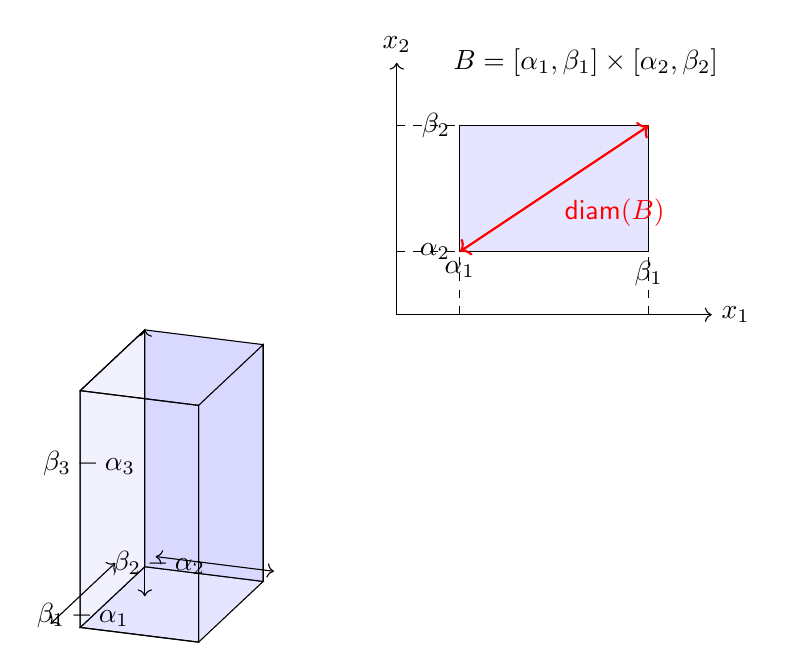
\begin{tikzpicture}[scale=0.8]
        % 3D Box
         % Box in R^2
         \draw[fill=blue!10] (5,5) rectangle (8,7);
         \draw[->] (4,4) -- (9,4) node[right]{$x_1$};
         \draw[->] (4,4) -- (4,8) node[above]{$x_2$};
         \draw[dashed] (5,4) -- (5,5) node[below]{$\alpha_1$};
         \draw[dashed] (8,4) -- (8,5) node[below]{$\beta_1$};
         \draw[dashed] (4,5) -- (5,5) node[left]{$\alpha_2$};
         \draw[dashed] (4,7) -- (5,7) node[left]{$\beta_2$};
         \node at (7,8) {$B = [\alpha_1,\beta_1] \times [\alpha_2,\beta_2]$};
         \draw[<->,red,thick] (5,5) -- node[midway,below right]{diam$(B)$} (8,7);
        \tdplotsetmaincoords{70}{110}
        \begin{scope}[tdplot_main_coords]
            \draw[fill=blue!10] (0,0,0) -- (3,0,0) -- (3,2,0) -- (0,2,0) -- cycle;
            \draw[fill=blue!5] (0,0,0) -- (0,0,4) -- (3,0,4) -- (3,0,0) -- cycle;
            \draw[fill=blue!15] (0,0,0) -- (0,2,0) -- (0,2,4) -- (0,0,4) -- cycle;
            \draw (3,0,0) -- (3,0,4) -- (3,2,4) -- (3,2,0) -- cycle;
            \draw (0,2,0) -- (0,2,4) -- (3,2,4) -- (3,2,0);
            \draw (0,0,4) -- (3,0,4) -- (3,2,4);
            \draw[<->] (0,-0.5,0) -- node[midway,below]{$\beta_1-\alpha_1$} (3,-0.5,0);
            \draw[<->] (-0.5,0,0) -- node[midway,left]{$\beta_2-\alpha_2$} (-0.5,2,0);
            \draw[<->] (0,0,-0.5) -- node[midway,left]{$\beta_3-\alpha_3$} (0,0,4);
        \end{scope}
    \end{tikzpicture}
\end{center}
\subsection*{Theorem}
Let $B \subseteq \mathbb{R}^{n}$ be a box, $\alpha, \beta \in \mathbb{R}$ and $f,g : B \rightarrow \mathbb{R}$ Riemann-integrable.
\begin{enumerate}
    \item Linearity: $\alpha f + \beta g$ is Riemann-integrable with \[\int_{B} (\alpha f + \beta g)(x) dx = \alpha \cdot \int_{B} f(x) dx + \beta \cdot \int_{B} g(x) dx\]
    \item Monotonicity: if $f(x) \leq g(x)$ for all $x \in B$, then \[\int_{B} f(x) dx \leq \int_{B} g(x) dx\]
    \item The function $x \mapsto |f(x)|$ is Riemann-integrable with \[\left\|\int_{B} f(x) dx\right\| \leq \int_{B} |f(x)| dx\]
    \item Every continuous function $h : B \rightarrow \mathbb{R}$ is Riemann-integrable
\end{enumerate}
\section{Fubini's Theorem (Satz von Fubini)}
\subsection*{Definition}
Let \( B = B(a,b) \subseteq \mathbb{R}^n \) be a box with \( a = (\alpha_1, \ldots,
\alpha_n)^T \in \mathbb{R}^n \) and \( b = (\beta_1, \ldots, \beta_n)^T \in \mathbb{R}^n \)
\\ and let \( f : B \to \mathbb{R} \) be a function on \( B \). For $i \in \left\{1,\cdots,n\right\}$
let \( a_{-i}, b_{-i} \) denote the vectors

\[ a_{-i} := (\alpha_1,\alpha_{2}, \cdots , \alpha_n)^T \in \mathbb{R}^{n-1} \] 
\[ b_{-i} := (\beta_1, \beta_2, \cdots , \beta_n)^T \in
\mathbb{R}^{n-1} \]

Then the function \[ F_i : B(a_{-i}, b_{-i}) \to \mathbb{R} \] defined by \[
F_{i+1} := \int_{x_i = \alpha_i}^{\beta_i} f(x_1, \dots, x_n) \, dx_i \] if \( x_i \) satisfies \[ x_i \in A
\]

is called the \textbf{i-th parameter} integral of \( F \) if it exists.
\subsection*{Theorem}
Let \( B(a,b) \subseteq \mathbb{R}^n \) be a box and \( f : B(a,b) \rightarrow \mathbb{R} \) be continuous on \( B(a,b) \).

\begin{enumerate}
    \item[(1)] The parameter integrals \( F_i \) are continuous on \( B(a_{-i}, b_{-i}) \) for \( i \in \left\{1, \cdots,n \right\} \).

    \item[(2)] Let \(\pi : \left\{1, \cdots,n\right\} \rightarrow \left\{1, \cdots, n\right\}\) be bijective (``punctuations''), then
    \[
    \int_{B(a,b)} f(x) dx = \int_{\alpha(\pi(1))}^{\beta(\pi(1))} \left( \int_{\alpha(\pi(2))}^{\beta(\pi(2))} \cdots \left( \int_{\alpha(\pi(n))}^{\beta(\pi(n))} f(x_1, x_2, \ldots, x_n) dx_{\pi(n)} \right) \cdots dx_{\pi(2)} \right) dx_{\pi(1)}
    \]
    for \( x_1, x_2, \ldots, x_n \in B(a,b) \).
\end{enumerate}

For continuous function \( f \) on a box \( B \) the integral \(\int_{B} f(x) dx\) can be computed through successive parametric integrals in arbitrary order.
\vspace{5mm}
\subsection{Integration over Arbitary Sets}
Let \( O \subseteq \mathbb{R}^n \), \( f: O \rightarrow \mathbb{R} \) and \( B \subseteq \mathbb{R}^n \) with \( O \subseteq B \) (i.e., \( O \) is bounded). Set  
\[ f_O : B \rightarrow \mathbb{R} \]  
\[ f_O(X) := 
\begin{cases} 
f(X), & x \in O; \\ 
0, & x \in B \setminus O.
\end{cases} \]

The function \( f \) is \textit{Riemann-integrable} over \( O \) if \( f_O \) is \textit{Riemann-integrable} over \( B \), and we set
\[ \int_{O} f(x) \, dx = \int_{B} f_O(x) \, dx. \]

A set \( D \subseteq \mathbb{R}^n \) is called \textit{Jordan-measurable} if the constant function \( x \mapsto 1 \) is integrable over \( D \); in that case, we denote the \( n \)-dimensional volume of \( D \) by
\[ \text{vol}(D) := \int_{D} 1 \, dx. \]

\subsection*{Example}
Consider the set of rational points in \([0, 1]^2\):
\[ Q := \{ x \in [0, 1]^2 : x \in \mathbb{Q}^2 \}. \]

\textbf{Volume of \( Q \)?}

\begin{itemize}
    \item Every box of positive diameter contains a rational point (because rationals are dense in the reals) and also an irrational point.
    \item Consider the characteristic function \( \chi_Q: [0, 1]^2 \rightarrow \mathbb{R} \),
    \[ \chi_Q(x) = 
    \begin{cases} 
    1, & x \in Q; \\ 
    0, & x \notin Q.
    \end{cases} \]
    \item For every partition, the supremum of \( \chi_Q \) over any sub-box is 1, and the infimum is 0.
    \item Thus, the upper Riemann sum is 1, and the lower Riemann sum is 0.
    \item \( \chi_Q \) is not Riemann-integrable over \([0, 1]^2\).
    \item \( Q \) is not Jordan-measurable.
\end{itemize}

\subsection{Normal Domains}
Consider sets with a "nice" description for integration.
A set \( O \subseteq \mathbb{R}^n \) is called a \textit{normal domain} if there exist two numbers \( \alpha \leq \beta \) and for each \( i \in \{1, \dots, n-1\} \) continuous functions \( \alpha_i, \beta_i: \mathbb{R}^i \rightarrow \mathbb{R} \), such that
\[ O = \left\{ x = \begin{pmatrix} x_1 \\ \vdots \\ x_n \end{pmatrix} : \alpha \leq x_1 \leq \beta \land \alpha_1(x_1) \leq x_2 \leq \beta_1(x_1) \land \dots \land \alpha_{n-1}(x_1, \dots, x_{n-1}) \leq x_n \leq \beta_{n-1}(x_1, \dots, x_{n-1}) \right\}. \]

\subsection*{Examples}
\begin{enumerate}
    \item 
    \[ D = \left\{ x = (x_1, x_2) \in \mathbb{R}^2 : -\frac{\sqrt{3}}{2} \leq x_1 \leq \frac{\sqrt{3}}{2} \land x_1^2 \leq x_2 \leq 7 - x_1^2 \right\}. \]
    This is a region bounded by two parabolas.

    \item 
    \[ D = \{ x \in \mathbb{R}^2 : \|x\|^2 \leq 7 \} \]
    This is a disc centered at the origin with radius \( \sqrt{7} \).

    \item 
    \[ D = \{ x \in \mathbb{R}^3 : \|x\|^2 \leq 7 \} \]
    This is a ball centered at the origin with radius \( \sqrt{7} \).
\end{enumerate}

\subsection{Theorem}
Let \( O \subseteq \mathbb{R}^n \) be a normal domain described by continuous functions \( \alpha, \beta \in \mathbb{R} \) and \( \alpha_i, \beta_i : \mathbb{R}^i \rightarrow \mathbb{R} \) for \( i \in \{1, \dots, n-1\} \). Then, a continuous function \( f: O \rightarrow \mathbb{R} \) is Riemann-integrable over \( O \) with
\[ \int_{O} f(x) \, dx = \int_{\alpha}^{\beta} \int_{\alpha_1(x_1)}^{\beta_1(x_1)} \cdots \int_{\alpha_{n-1}(x_1, \dots, x_{n-1})}^{\beta_{n-1}(x_1, \dots, x_{n-1})} f(x_1, \dots, x_n) \, dx_n \cdots dx_1. \]
\newpage
\subsection{Change of Variables}
    Let \( X \subseteq \mathbb{R}^n \) be open and \( g : X \to \mathbb{R}^n \) an injective, continuously differentiable function with  
    \[ \det(J_g(x)) \neq 0 \quad \text{for all } x \in X, \]  
    where \( J_g(x) \) is the Jacobian matrix of \( g \) at \( x \).
    
    \begin{enumerate}[label=(\arabic*)]
        \item If \( D \subseteq X \) is closed, bounded, and Jordan-measurable, then \( g(D) \) is also closed, bounded, and Jordan-measurable.
        
        \item Let \( D \subseteq X \) be closed, bounded, and Jordan-measurable, and let \( f : g(D) \to \mathbb{R} \) be continuous. Then \( f \) is Riemann-integrable over \( g(D) \), and  
        \[ \int_{g(D)} f(y) \, dy = \int_{D} f(g(x)) \cdot |\det(J_g(x))| \, dx. \]
    \end{enumerate}

    
    \subsection*{Examples of Transformations (Polar-, Kugel-, Zylinderkoordinaten)}
    
    \subsubsection{Half-Ring in Polar Coordinates}
    \[ X = \{x \in \mathbb{R}^2 : x_1 > 0, \, 1 < \|x\|^2 < 4\}, \]  
    \[ f(x_1, x_2) = x_1 \cdot (x_1^2 + x_2^2). \]  
    This is a half-ring with inner radius \( 1 \) and outer radius \( 2 \).  
    
    In polar coordinates:  
    \[ X = \left\{ (x_1, x_2) = (r \cos t, r \sin t) : 1 < r < 2, \, -\frac{\pi}{2} < t < \frac{\pi}{2} \right\}. \]  
    The variables \( r \) and \( t \) are independent, making \( X \) a "box" in polar coordinates.
    
    \subsubsection{Transformation and Jacobian}
    To evaluate \( \int_X x \, dx \) using polar coordinates:  
    \[ g(r, t) = \begin{pmatrix} r \cos t \\ r \sin t \end{pmatrix}, \]  
    with domain \( D = \{(r, t) : r \in (1, 2), \, t \in (-\frac{\pi}{2}, \frac{\pi}{2})\} \).  
    
    The Jacobian matrix of \( g \) is:  
    \[ J_g(r, t) = \begin{pmatrix} \cos t & -r \sin t \\ \sin t & r \cos t \end{pmatrix}, \]  
    and its determinant is \( \det(J_g(r, t)) = r \).
    
    \subsubsection{Octant of a Ball in Spherical Coordinates}
    \[ X = \{ x \in \mathbb{R}^3 : x_1, x_2, x_3 \geq 0, \, x_1^2 + x_2^2 + x_3^2 \leq 1 \}. \]  
    This is the first octant of a ball with radius \( \sqrt{7} \).  
    
    In spherical coordinates:  
    \[ g(r, \rho, \psi) = \begin{pmatrix} r \cos \rho \cos \psi \\ r \sin \rho \cos \psi \\ r \sin \psi \end{pmatrix}, \]  
    with \( D = \{(r, \rho, \psi) : r \in (0, \sqrt{1}), \, \rho \in (0, \frac{\pi}{2}), \, \psi \in (0, \frac{\pi}{2})\} \).  
    
    The Jacobian determinant is:  
    \[ \det(J_g(r, \rho, \psi)) = r^2 \cos \psi. \]  
    
    The volume integral becomes:  
    \[ \int_X 1 \, dx = \int_{r=0}^{\sqrt{1}} \int_{\rho=0}^{\pi/2} \int_{\psi=0}^{\pi/2} r^2 \cos \psi \, d\psi \, d\rho \, dr. \]
    
    \subsection{Parametrized Curves}
    
    \subsubsection*{Definition}
    A \textit{parametrized curve} in \( \mathbb{R}^n \) is a continuous, piecewise continuously differentiable mapping \( \gamma : I \to \mathbb{R}^n \), where \( I \subseteq \mathbb{R} \) is an interval. The \textit{graph} (or trace) of \( \gamma \) is the set:  
    \[ \text{graph}(\gamma) = \{\gamma(t) : t \in I\}. \]  
    
    For \( t \in I \) where \( \gamma \) is differentiable:  
    \begin{itemize}
        \item The derivative \( \gamma'(t) \) is called the \textit{tangent vector} of \( \gamma \) at \( t \).
        \item The norm \( \|\gamma'(t)\| \) is called the \textit{speed} of \( \gamma \) at \( t \).
    \end{itemize}
    
    \subsection{Examples}
    \begin{enumerate}
        \item Linear path:  
        \[ \gamma : [0, 7] \to \mathbb{R}^2, \quad \gamma(t) = \begin{pmatrix} t \\ t \end{pmatrix}. \]  
        
        \item Quadratic path:  
        \[ \gamma : [0, 7] \to \mathbb{R}^2, \quad \gamma(t) = \begin{pmatrix} t^2 \\ t^2 \end{pmatrix}. \]  
        
        \item Unit circle:  
        \[ \gamma : [0, 2\pi] \to \mathbb{R}^2, \quad \gamma(t) = \begin{pmatrix} \cos t \\ \sin t \end{pmatrix}. \]  
        The speed is constant: \( \|\gamma'(t)\| = 1 \).  
        
        \item Decaying spiral:  
        \[ \gamma : [0, \infty) \to \mathbb{R}^2, \quad \gamma(t) = e^{-t} \begin{pmatrix} \cos t \\ \sin t \end{pmatrix}. \]  
        
        \item Graph of a function:  
        For \( f : [\alpha, \beta] \to \mathbb{R} \Rightarrow \gamma_f : [\alpha,\beta] \rightarrow \mathbb{R}^{2}\),  
        \[ \gamma_f(t) = \begin{pmatrix} t \\ f(t) \end{pmatrix}. \]  
        
        \item Helix:  
        \[ \gamma : [0, \infty) \to \mathbb{R}^3, \quad \gamma(t) = \begin{pmatrix} \cos t \\ \sin t \\ t \end{pmatrix}. \]  
    \end{enumerate}
\subsection{Curve Length}

For a parametrized curve \(\gamma : I \rightarrow \mathbb{R}^n\), we assume:
\[ \dot{\gamma}(t) \neq 0 \text{ for all } t \in I. \]

\begin{itemize}
    \item Let \(\gamma : [\alpha, \beta] \rightarrow \mathbb{R}^n\) be a curve.
    \item Partition the interval \([\alpha, \beta]\) with points:
    \[ \alpha = t_0 < t_1 < \cdots < t_{n-1} < t_n = \beta. \]
    \item Compute the length of the polygonal path through \(\gamma(t_0), \gamma(t_1), \ldots, \gamma(t_n)\):
    \[ L_n = \sum_{k=1}^n \|\gamma(t_k) - \gamma(t_{k-1})\|. \]
    \item This approximates the true curve length \(s(\gamma)\).
    \item Rewrite using the mean value theorem:
    \[ L_n = \sum_{k=1}^n (t_k - t_{k-1}) \cdot \left\|\frac{\gamma(t_k) - \gamma(t_{k-1})}{t_k - t_{k-1}}\right\|. \]
    \item As the partition becomes finer (\(|t_k - t_{k-1}| \rightarrow 0\)):
    \[ s(\gamma) = \int_{\alpha}^{\beta} \|\dot{\gamma}(t)\| \, dt. \]
\end{itemize}

\subsubsection{Theorem}
Let \(\gamma: [\alpha, \beta] \rightarrow \mathbb{R}^n\) be a continuously differentiable curve with \(\dot{\gamma}(t) \neq 0\) for all \(t \in [\alpha, \beta]\). Then the length \(s(\gamma)\) of the curve is:
\[ s(\gamma) = \int_{\alpha}^{\beta} \|\dot{\gamma}(t)\| \, dt. \]

\textbf{Example: Logarithmic Spiral} \\
Consider the logarithmic spiral:
\[ \gamma: [0, \infty) \rightarrow \mathbb{R}^2, \quad \gamma(t) = e^{-t} \begin{pmatrix} \cos t \\ \sin t \end{pmatrix}. \]

\[ \dot{\gamma}(t) = e^{-t} \begin{pmatrix} -\cos t - \sin t \\ -\sin t + \cos t \end{pmatrix}. \]

\begin{align*}
\|\dot{\gamma}(t)\| &= e^{-t} \sqrt{(-\cos t - \sin t)^2 + (-\sin t + \cos t)^2} \\
&= e^{-t} \sqrt{(\cos^2 t + 2\cos t \sin t + \sin^2 t) + (\cos^2 t - 2\cos t \sin t + \sin^2 t)} \\
&= e^{-t} \sqrt{2(\cos^2 t + \sin^2 t)} \\
&= e^{-t} \sqrt{2}.
\end{align*}

\[ s(\gamma) = \int_0^\infty \|\dot{\gamma}(t)\| \, dt = \sqrt{2} \int_0^\infty e^{-t} \, dt = \sqrt{2} \left[ -e^{-t} \right]_0^\infty = \sqrt{2}. \]


We want to define functions using polar coordinates in the plane:
\begin{itemize}
    \item Domain: Angle $\theta$
    \item Function value: Radius $r = r(\theta)$
    \item Typically, domain is an interval of $[0,2\pi)$ (or a translation)
    \item Recall the polar-to-Cartesian transformation:
    \[ T(r,\theta) = \begin{pmatrix} r\cos\theta \\ r\sin\theta \end{pmatrix} \]
\end{itemize}

\subsection*{Definition}
Let $I \subseteq [0,2\pi)$ and let $r: I \rightarrow \mathbb{R}_{\geq 0}$ be a continuous function. The curve $\gamma: I \rightarrow \mathbb{R}^2$ defined by
\[ \gamma(\theta) := T(r(\theta), \theta) \]
is the \textit{polar curve} associated to $r$, where $T$ is the transformation from polar to Cartesian coordinates.

\subsection*{Examples}
\begin{enumerate}[label=(\alph*)]
    \item A circle with radius $r^* \in \mathbb{R}_{>0}$ is a polar curve:
    \[ \gamma: [0, 2\pi) \rightarrow \mathbb{R}^2, \quad \gamma(\theta) = \begin{pmatrix} r^*\cos\theta \\ r^*\sin\theta \end{pmatrix} = T(r^*, \theta) \]
    or equivalently:
    \[ r(\theta) := r^* \]
    
    \item Rose petal curve:
    \[ r(\theta) = 3\sin(2\theta), \quad \theta \in \left[0, \frac{\pi}{2}\right) \]
\end{enumerate}


For a circle:
\[ \text{Area} = \frac{r^2}{2}(\theta_2 - \theta_1) \]
This represents the ratio of the sector angle to the full circle:
\[ \frac{\theta_2 - \theta_1}{2\pi} \times \pi r^2 = \frac{r^2}{2}(\theta_2 - \theta_1) \]

\subsection{General Polar Curve}
For a polar curve with radius $r = r(\theta)$:
\begin{itemize}
    \item Subdivide the angle interval $[\theta_1, \theta_2]$
    \item Approximate area using circular sectors:
    \[ \text{Area} \approx \sum_{i=1}^{n-1} \frac{[r(\theta_i)]^2}{2} \cdot (\theta_{i+1} - \theta_i) \]
    \item Take the limit as the partition becomes finer (Riemann sum):
    \[ \text{Area} = \int_{\theta_1}^{\theta_2} \frac{[r(\theta)]^2}{2} \, d\theta \]
\end{itemize}

For a planar curve in polar coordinates, the sector area between angles $\theta_1$ and $\theta_2$ is given by:
\[ A = \frac{1}{2}\int_{\theta_1}^{\theta_2} [r(\theta)]^2 d\theta \]

\vspace{5mm}
Consider a curve $\gamma: I \rightarrow \mathbb{R}^2$ given in Cartesian coordinates:
\[ \gamma(t) = \begin{pmatrix} x_1(t) \\ x_2(t) \end{pmatrix} \]

\[
\int_{t_1}^{t_2} f(g(t)) \cdot g'(t) dt = \int_{g(t_1)}^{g(t_2)} f(x)
\]

area can be written as 
\[
\int_{t_1}^{t_2} \frac{1}{2} [r(\rho(t))]^{2} \cdot \dot{\rho}(t) dt 
\]

Using the polar transformation:
\[ T(r,\theta) = \begin{pmatrix} r\cos\theta \\ r\sin\theta \end{pmatrix} \]
\newpage
We can extract polar coordinates from Cartesian coordinates:
\begin{align*}
r(t)^2 &= x_1(t)^2 + x_2(t)^2 \\
\theta(t) &= \arctan\left(\frac{x_2(t)}{x_1(t)}\right)
\end{align*}


The derivative of $\theta(t)$ is:
\begin{align*}
\frac{d}{dt}\theta(t) &= \frac{d}{dt}\left(\arctan\frac{x_2(t)}{x_1(t)}\right) \\
&= \frac{1}{1 + \left(\frac{x_2(t)}{x_1(t)}\right)^2} \cdot \frac{\dot{x}_2(t)x_1(t) - x_2(t)\dot{x}_1(t)}{x_1(t)^2} \\
&= \frac{\dot{x}_2(t)x_1(t) - x_2(t)\dot{x}_1(t)}{x_1(t)^2 + x_2(t)^2}
\end{align*}

For a general parametric curve, the sector area between parameters $t_1$ and $t_2$ is:
\begin{align*}
A &= \frac{1}{2}\int_{t_1}^{t_2} [r(\theta(t))]^2 \dot{\theta}(t) dt \\
&= \frac{1}{2}\int_{t_1}^{t_2} \left(x_1(t)^2 + x_2(t)^2\right) \cdot \frac{\dot{x}_2(t)x_1(t) - x_2(t)\dot{x}_1(t)}{x_1(t)^2 + x_2(t)^2} dt \\
&= \frac{1}{2}\int_{t_1}^{t_2} \left(\dot{x}_2(t)x_1(t) - x_2(t)\dot{x}_1(t)\right) dt
\end{align*}

This represents the sector area of the planar curve $\gamma(t) = \begin{pmatrix} x_1(t) \\ x_2(t) \end{pmatrix}$ between parameters $t_1$ and $t_2$.
\vspace{5mm}
\section{Line Integrals}
Consider a function \( f : \mathbb{R}^n \rightarrow \mathbb{R} \) and a curve
\[ \gamma : [\alpha, \beta] \rightarrow \mathbb{R}^n. \]
We would like to compute the integral of \( f \) along \( \gamma \) - called the \textit{line integral}.

\subsection*{Definition}
Let \( f: \mathbb{R}^n \to \mathbb{R} \) be a scalar function and 
\( \gamma : [\alpha, \beta] \to \mathbb{R}^n \) be a curve. The line integral of \( f \) along \( \gamma \) is defined as:
\[ \int_{\gamma} f \, ds := \int_{\alpha}^{\beta} f(\gamma(t)) \cdot \|\dot{\gamma}(t)\| \, dt. \]

\begin{itemize}
    \item \( ds \) represents the arc length element
    \item If \( \gamma \) is closed (i.e., \( \gamma(\alpha)=\gamma(\beta) \)), we denote the integral with a circle: \( \oint_{\gamma} f \, ds \)
\end{itemize}

Approximate the curve with a polygonal path through points:
\[ \gamma(t_1), \gamma(t_2), \ldots, \gamma(t_n) \]
where \( \alpha = t_0 < t_1 < \cdots < t_n = \beta \).

The Riemann sum approximation is:
\[ \sum_{k=1}^n f(\gamma(t_k)) \cdot \|\gamma(t_k) - \gamma(t_{k-1})\| \]
\[ = \sum_{k=1}^n f(\gamma(t_k)) \cdot \left\|\frac{\gamma(t_k) - \gamma(t_{k-1})}{t_k - t_{k-1}}\right\| \cdot (t_k - t_{k-1}) \]

Taking the limit as the partition becomes finer yields the integral:
\[ \int_{\alpha}^{\beta} f(\gamma(t)) \cdot \|\dot{\gamma}(t)\| \, dt \]

\subsection*{Example}
Consider:
\begin{align*}
f : \mathbb{R}^3 &\to \mathbb{R} \\
f(x_1, x_2, x_3) &= x_1^2 + x_2 \cdot x_3
\end{align*}

and the helical curve:
\[ \gamma : [0, 2\pi] \to \mathbb{R}^3, \quad \gamma(t) = \begin{pmatrix} \cos t \\ \sin t \\ t \end{pmatrix} \]

1. Compute the derivative:
\[ \dot{\gamma}(t) = \begin{pmatrix} -\sin t \\ \cos t \\ 1 \end{pmatrix} \]
\[ \|\dot{\gamma}(t)\| = \sqrt{(-\sin t)^2 + \cos^2 t + 1^2} = \sqrt{2} \]

2. Compute the line integral:
\begin{align*}
\int_{\gamma} f \, ds &= \int_{0}^{2\pi} f(\gamma(t)) \cdot \|\dot{\gamma}(t)\| \, dt \\
&= \sqrt{2} \int_{0}^{2\pi} (\cos^2 t + t \sin t) \, dt \\
&= \sqrt{2} \left( \int_{0}^{2\pi} \cos^2 t \, dt + \int_{0}^{2\pi} t \sin t \, dt \right)
\end{align*}

3. Evaluate each integral:
\begin{itemize}
    \item For \( \cos^2 t \):
    \[ \int \cos^2 t \, dt = \frac{1}{2}(\cos t \sin t + t) + C \]
    \[ \left. \frac{1}{2}(\cos t \sin t + t) \right|_{0}^{2\pi} = \pi \]
    
    \item For \( t \sin t \):
    \[ \int t \sin t \, dt = -t \cos t + \sin t + C \]
    \[ \left. (-t \cos t + \sin t) \right|_{0}^{2\pi} = -2\pi \]
\end{itemize}

4. Final result:
\[ \int_{\gamma} f \, ds = \sqrt{2}(\pi - 2\pi) = -\pi\sqrt{2} \]
\vspace{5mm}
\subsection{Vector Fields}
Vector fields describe quantities with both magnitude and direction that may vary depending on location in space.

\subsubsection{Examples}
\begin{itemize}
    \item Varying winds in the atmosphere
    \item Ocean currents
    \item Gravitational field acting on a satellite
    \item Motion of charged particles in electromagnetic fields
\end{itemize}

\subsubsection{Definitions}
A set \( O \subseteq \mathbb{R}^n \) is called \textit{connected} if for any two points \( x, y \in O \), there exists a continuous curve connecting \( x \) to \( y \) that lies entirely within \( O \).

Let \( O \subseteq \mathbb{R}^n \) be connected. A function \( v : O \to \mathbb{R}^n \) is called an \textit{n-dimensional vector field} over \( O \). In contrast, \( f : O \to \mathbb{R} \) is called a \textit{scalar field}.

Vector fields can be visualized by plotting vectors \( v(X_i) \) anchored at sample points \( X_i \in D \) (typically a regular grid).
\\
\textbf{Examples of Vector Fields}
\begin{enumerate}
    \item \textbf{Constant Field}:
    \[ v : \mathbb{R}^2 \to \mathbb{R}^2, \quad v(x_1, x_2) = \begin{pmatrix} 1 \\ 1 \end{pmatrix} \]
    
    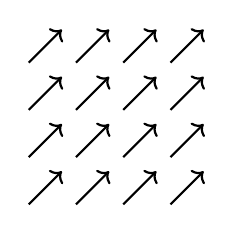
\begin{tikzpicture}[scale=0.6]
        \foreach \x in {0,1,2,3}
            \foreach \y in {0,1,2,3}
                \draw[->, thick] (\x,\y) -- (\x+0.7,\y+0.7);
    \end{tikzpicture}
    
    \item \textbf{Central Field}:
    \[ V : \mathbb{R}^2 \to \mathbb{R}^2, \quad V\begin{pmatrix} x_1 \\ x_2 \end{pmatrix} = -\frac{1}{\|x\|^2} \begin{pmatrix} x_1 \\ x_2 \end{pmatrix} \]
    where \( \|x\| = \sqrt{x_1^2 + x_2^2} \).
    
    \item \textbf{Rotational Field}:
    \[ V : \mathbb{R}^2 \to \mathbb{R}^2, \quad V\begin{pmatrix} x_1 \\ x_2 \end{pmatrix} = \begin{pmatrix} -x_2 \\ x_1 \end{pmatrix} \]
    Note that \( V(x) \perp x \) for all \( x \).
    
    \item \textbf{Gradient Field}:
    Let \( F: \mathbb{R}^n \to \mathbb{R} \) be differentiable. The gradient field is:
    \[ v(x) = \nabla F(x) = \begin{pmatrix} \frac{\partial F}{\partial x_1} \\ \vdots \\ \frac{\partial F}{\partial x_n} \end{pmatrix} \]
    
    \textbf{Example}:
    \[ F(x_1,x_2) = x_1^2 + x_2^2 \]
    \[ \nabla F(x) = \begin{pmatrix} 2x_1 \\ 2x_2 \end{pmatrix} = 2x \]
\end{enumerate}

\subsection{Rotation and Divergence}
\subsubsection*{Definition}
Let $v : \mathbb{R}^{3} \rightarrow \mathbb{R}^{3}$ be differentiable, then the \textbf{rotation (rotor) of v} is the vector field \textbf{rot}$(v)$ defined as:
\[
\text{rot } v = \begin{pmatrix} \dfrac{\partial v_3}{\partial x_2} - \dfrac{\partial v_2}{\partial x_3} \\ \dfrac{\partial v_1}{\partial x_3} - \dfrac{\partial v_3}{\partial x_1} \\ \dfrac{\partial v_2}{\partial x_1} - \dfrac{\partial v_1}{\partial x_2} \end{pmatrix} 
\]
memory aid: 
\[
\text{rot } v = \begin{pmatrix} \dfrac{\partial}{\partial x_1} \\ \dfrac{\partial}{\partial x_2} \\ \dfrac{\partial}{\partial x_3} \end{pmatrix} \times \begin{pmatrix} v_1 \\ v_2 \\ v_3 \end{pmatrix}
\]
rot $v$ is the measure for local rotation of a vector field as experienced by a partial moving along the field
\subsubsection*{Definition}
Let $v : \mathbb{R}^{n} \rightarrow \mathbb{R}^{n}$ be differentiable, then the \textbf{diversion of v} is the function: 
\[
\text{div} v(x) = \sum_{i = 1}^{n} \dfrac{\partial v_i}{\partial x_i}(x)
\]
memory aid: 
\[
\text{div } v = \langle\nabla, v\rangle = \langle \begin{pmatrix} \dfrac{\partial}{\partial x_1} \\ \vdots \\ \dfrac{\partial}{\partial x_n} \end{pmatrix} , \begin{pmatrix} v_1 \\ \vdots \\ v_n \end{pmatrix} \rangle
\]
divergence is a measure of local density of sources/sinks
\section{Line Integrals over Vector Fields}
A vector field \( v: \mathbb{R}^n \to \mathbb{R}^n \) (e.g., gravitational, electric/magnetic field, wind, etc.) is given.

\begin{itemize}
    \item A curve \( \gamma: [a, b] \to \mathbb{R}^n \) describes a motion through \( v \) under the influence of the field described by \( v \) (e.g., movement of an airplane through atmospheric wind).
    \item What is the amount of energy necessary for that movement?
    \item What is the amount of work expended at this point (amount of field \( v \) that winds in air)?
\end{itemize}

\subsection{Line Integral}
The line integral is the projection of \( v(x) \) onto the direction of movement \( \dot{\gamma}(t) \) where \( \gamma(t) = x \).

\begin{itemize}
    \item Effective strength of the force at point \( x \) that is experienced when moving along curve \( \gamma \) at point \( x \).
    \item Integrable projection of \( v(\gamma(t)) \) onto \( \dot{\gamma}(t) \) along the curve \( \gamma \).
    \item Projection (line integral): \( \langle v(\gamma(t)), \frac{\dot{\gamma}(t)}{\|\dot{\gamma}(t)\|} \rangle \) for absolute \( t \) (includes sign).
\end{itemize}

The line integral can be written as:
\[
\int_{\gamma} f \, ds = \int_{a}^{b} \langle v(\gamma(t)), \frac{\dot{\gamma}(t)}{\|\dot{\gamma}(t)\|} \rangle \|\dot{\gamma}(t)\| \, dt = \int_{a}^{b} \langle v(\gamma(t)), \dot{\gamma}(t) \rangle \, dt
\]

\subsection*{Definition}
Let \( v: D \to \mathbb{R}^n \) be a vector field on a connected set \( D \subseteq \mathbb{R}^n \), and let \( \gamma: [a, b] \to D \) be a curve contained in \( D \). The line integral of \( v \) along \( \gamma \), denoted by \( \int_{\gamma} v \, ds \), is defined as:
\[
\int_{\gamma} v \, ds = \int_{a}^{b} \langle v(\gamma(t)), \dot{\gamma}(t) \rangle \, dt
\]

\subsection*{Example}
Let \( v: \mathbb{R}^3 \to \mathbb{R}^3 \) be defined by:
\[
v \begin{pmatrix} x_1 \\ x_2 \\ x_3 \end{pmatrix} = \begin{pmatrix} x_1 x_2^2 \\ x_1 x_3 \\ x_3 \end{pmatrix}
\]
Let \( \gamma: [0, 1] \to \mathbb{R}^3 \) be defined by:
\[
\gamma(t) = \begin{pmatrix} t \\ t^2 \\ t^3 \end{pmatrix}
\]
The line integral of \( v \) along \( \gamma \) is:
\[
\int_{\gamma} v \, ds = \int_{0}^{1} \langle v(\gamma(t)), \dot{\gamma}(t) \rangle \, dt
\]
First, compute \( v(\gamma(t)) \):
\[
v(\gamma(t)) = v \begin{pmatrix} t \\ t^2 \\ t^3 \end{pmatrix} = \begin{pmatrix} t \cdot (t^2)^2 \\ t \cdot t^3 \\ t^3 \end{pmatrix} = \begin{pmatrix} t^5 \\ t^4 \\ t^3 \end{pmatrix}
\]
Next, compute \( \dot{\gamma}(t) \):
\[
\dot{\gamma}(t) = \begin{pmatrix} 1 \\ 2t \\ 3t^2 \end{pmatrix}
\]
Now, compute the dot product:
\[
\langle v(\gamma(t)), \dot{\gamma}(t) \rangle = t^5 \cdot 1 + t^4 \cdot 2t + t^3 \cdot 3t^2 = t^5 + 2t^5 + 3t^5 = 6t^5
\]
Finally, integrate:
\[
\int_{0}^{1} 6t^5 \, dt = \left[ t^6 \right]_{0}^{1} = 1
\]
\subsection{Gradient Fields}
For a scalar field \( F : D \rightarrow \mathbb{R} \), the gradient defines a vector field:
\[
\text{grad } F : D \rightarrow \mathbb{R}^n, \quad \text{grad } F(x) = \nabla F(x).
\]
One could say that \( F \) is an antiderivative of the vector field \( \text{grad } F \). Vector fields that can be represented as the gradient of some scalar field have a special name.

\subsection*{Definition}
A vector field \( v: D \rightarrow \mathbb{R}^n \) on a connected set \( D \subseteq \mathbb{R}^n \) is called a \textbf{gradient field}, \textbf{potential field}, or \textbf{conservative} if there exists a scalar field \( F: D \rightarrow \mathbb{R} \) such that:
\[
v = \text{grad } F.
\]
Such a function \( F \) is called a \textbf{potential} or an \textbf{antiderivative} of \( v \).
\\
\textbf{Example 1}\\
Consider the vector field:
\[
v \begin{pmatrix} x_1 \\ x_2 \\ x_3 \end{pmatrix} = 
\begin{pmatrix} 
x_2 e^{x_1 x_2 + x_3} \\ 
x_1 e^{x_1 x_2} \\ 
x_1 + 2 x_3 
\end{pmatrix}.
\]
Is \( v \) a gradient field?

Assume there exists a potential \( F: \mathbb{R}^3 \rightarrow \mathbb{R} \) such that \( v = \text{grad } F \). Then:
\[
\frac{\partial F}{\partial x_1}(x) = x_2 e^{x_1 x_2 + x_3}, \quad
\frac{\partial F}{\partial x_2}(x) = x_1 e^{x_1 x_2}, \quad
\frac{\partial F}{\partial x_3}(x) = x_1 + 2 x_3.
\]

Integrate the first equation with respect to \( x_1 \):
\[
F(x) = \int x_2 e^{x_1 x_2 + x_3} \, dx_1 = e^{x_1 x_2 + x_3} + \Phi_1(x_2, x_3).
\]
But from the second equation:
\[
\frac{\partial F}{\partial x_2}(x) = x_1 e^{x_1 x_2} = x_1 e^{x_1 x_2} + \frac{\partial}{\partial x_2} \Phi_1(x_2, x_3).
\]
This implies:
\[
\frac{\partial}{\partial x_2} \Phi_1(x_2, x_3) = 0 \Rightarrow \Phi_1 \text{ does not depend on } x_2.
\]
Thus, \( \Phi_1(x_2, x_3) = \Phi_2(x_3) \), and:
\[
F(x) = e^{x_1 x_2 + x_3} + \Phi_2(x_3).
\]
Now, from the third equation:
\[
\frac{\partial F}{\partial x_3}(x) = e^{x_1 x_2 + x_3} + \frac{d}{dx_3} \Phi_2(x_3) = x_1 + 2 x_3.
\]
This requires:
\[
\frac{d}{dx_3} \Phi_2(x_3) = x_1 + 2 x_3 - e^{x_1 x_2 + x_3},
\]
which is impossible unless \( x_1 x_2 + x_3 \) is constant. Therefore, \( v \) is \textbf{not} a gradient field.
\\
\textbf{Example 2}\\
Consider the vector field:
\[
v \begin{pmatrix} x_1 \\ x_2 \\ x_3 \end{pmatrix} = 
\begin{pmatrix}
x_2 e^{x_1} + x_2 x_3 \\
e^{x_1} + x_1 x_3 \\
e^{x_1} + x_1 x_2
\end{pmatrix}.
\]
Assume there exists a potential \( F: \mathbb{R}^3 \rightarrow \mathbb{R} \) for \( v \). Then:
\[
\frac{\partial F}{\partial x_1}(x) = x_2 e^{x_1} + x_2 x_3 \Rightarrow F(x) = x_2 e^{x_1} + x_1 x_2 x_3 + \Phi_1(x_2, x_3).
\]
From the second equation:
\[
\frac{\partial F}{\partial x_2}(x) = e^{x_1} + x_1 x_3 + \frac{\partial}{\partial x_2} \Phi_1(x_2, x_3) = e^{x_1} + x_1 x_3.
\]
This implies:
\[
\frac{\partial}{\partial x_2} \Phi_1(x_2, x_3) = 0 \Rightarrow \Phi_1 \text{ does not depend on } x_2.
\]
Thus, \( \Phi_1(x_2, x_3) = \Phi_2(x_3) \), and:
\[
F(x) = x_2 e^{x_1} + x_1 x_2 x_3 + \Phi_2(x_3).
\]
Now, from the third equation:
\[
\frac{\partial F}{\partial x_3}(x) = x_1 x_2 + \frac{d}{dx_3} \Phi_2(x_3) = e^{x_1} + x_1 x_2.
\]
This requires:
\[
\frac{d}{dx_3} \Phi_2(x_3) = e^{x_1},
\]
which is impossible because \( \Phi_2 \) depends only on \( x_3 \), not on \( x_1 \). Therefore, \( v \) is \textbf{not} conservative.

\subsection{Line Integrals in Gradient Fields}
Consider a gradient field \( v: \mathbb{R}^n \rightarrow \mathbb{R}^n \) with potential \( F : \mathbb{R}^n \rightarrow \mathbb{R} \) and a curve \( \gamma : [\alpha, \beta] \rightarrow \mathbb{R}^n \) with \( a = \gamma(\alpha) \) and \( b = \gamma(\beta) \). Then:
\[
\text{grad } F(x) = v(x) \quad \forall x \in \mathbb{R}^n.
\]
Define the function \( f(t) := F(\gamma(t)) \), the restriction of \( F \) to the curve \( \gamma \). Then:
\[
f'(t) = \nabla F(\gamma(t)) \cdot \dot{\gamma}(t) = \langle v(\gamma(t)), \dot{\gamma}(t) \rangle.
\]
Thus, the line integral of \( v \) along \( \gamma \) is:
\[
\int_{\gamma} v \, ds = \int_{\alpha}^{\beta} \langle v(\gamma(t)), \dot{\gamma}(t) \rangle \, dt = \int_{\alpha}^{\beta} f'(t) \, dt = f(\beta) - f(\alpha) = F(b) - F(a).
\]
This shows that the line integral depends only on the potential \( F \) and its values at the endpoints of \( \gamma \).
\newpage
\subsection{Theorem}
Let $ D \subseteq \mathbb{R}^{n}$ be open, $v : D \rightarrow \mathbb{R}^{n}$ a continuous vector field on $D$ and $\gamma : (\alpha, \beta) \rightarrow D$ a continously differentiable curve. If $v$ is a gradient field, then the value of the line integral $\int_{gamma} v ds$ only depends only on the start- and endpoint of $\gamma$:
\[
\int_{\gamma} v ds = F(\gamma(\beta)) - F(\gamma(\alpha))
\]
where $F : D \rightarrow \mathbb{R}$ is a potential of $v$ \\
In particular, if $\gamma$ is a closed curve, i.e. $\gamma(\beta) = \gamma(\alpha)$, then \[\int_{\gamma} v ds = 0\]
\vspace{5mm}
\section{Integrability Conditions (Integrablitätsbedingungen)}
Let \( F : D \rightarrow \mathbb{R} \) be a potential for a differentiable vector field \( v : D \rightarrow \mathbb{R}^n \).

If \( F \in C^2 \), then by Schwarz's Theorem:
\[
\frac{\partial^2 F}{\partial x_i \partial x_j} (x) = \frac{\partial^2 F}{\partial x_j \partial x_i} (x) \quad \text{for all } i \neq j
\]
This implies the integrability conditions for \( v \):
\[
\frac{\partial v_j}{\partial x_i} (x) = \frac{\partial v_i}{\partial x_j} (x) \quad \text{for all } i \neq j
\]

\subsection*{Theorem}
Let \( v: D \rightarrow \mathbb{R}^n \) be a continuously differentiable vector field. If \( v \) is a gradient field, then:
\[
\frac{\partial v_j}{\partial x_i}(x) = \frac{\partial v_i}{\partial x_j}(x) \quad \text{for all } i,j \in \{1,\dots,n\} \text{ with } i \neq j.
\]

\subsection*{Simply Connected Domains}
A connected set \( D \subseteq \mathbb{R}^n \) is called \textbf{simply connected} if every closed curve in \( D \) can be continuously contracted to a single point in \( D \). Every convex set is simply connected.

\subsection*{Example 1}
Consider \( v : \mathbb{R}^2 \to \mathbb{R}^2 \):
\[
v(x_1, x_2) = \begin{pmatrix} -x_2 \\ x_1 \end{pmatrix}
\]
Check integrability conditions:
\[
\frac{\partial v_1}{\partial x_2} = -1, \quad \frac{\partial v_2}{\partial x_1} = +1
\]
Since \(-1 \neq +1\), \( v \) is \textbf{not} a gradient field on \( \mathbb{R}^2 \).

\subsection*{Example 2}
Consider \( v : \mathbb{R}^2 \to \mathbb{R}^2 \):
\[
v(x_1, x_2) = \begin{pmatrix} x_1 \\ x_2 \end{pmatrix}
\]
Integrability conditions:
\[
\frac{\partial v_1}{\partial x_2} = 0 = \frac{\partial v_2}{\partial x_1}
\]
Since \( \mathbb{R}^2 \) is simply connected, \( v \) \textbf{is} a gradient field.

\subsection*{Example 3}
Consider \( v : \mathbb{R}^2 \setminus \{0\} \to \mathbb{R}^2 \):
\[
v(x_1, x_2) = \frac{1}{x_1^2 + x_2^2} \begin{pmatrix} -x_2 \\ x_1 \end{pmatrix}
\]
Integrability conditions:
\[
\frac{\partial v_1}{\partial x_2} = \frac{-x_1^2 + x_2^2}{(x_1^2 + x_2^2)^2} = \frac{\partial v_2}{\partial x_1}
\]
The domain \( \mathbb{R}^2 \setminus \{0\} \) is \textbf{not} simply connected, so we cannot conclude that \( v \) is a gradient field. However, if we restrict to a simply connected subdomain (not containing the origin), then \( v \) has a potential.

\subsection*{Example 4}
Consider \( v : \mathbb{R}^3 \rightarrow \mathbb{R}^3 \):
\[
v(x_1, x_2, x_3) = \begin{pmatrix} e^{x_1} x_2 \\ e^{x_1} x_1 \\ x_3 \end{pmatrix}
\]
Integrability conditions:
\[
\frac{\partial v_1}{\partial x_2} = e^{x_1} = \frac{\partial v_2}{\partial x_1}, \quad
\frac{\partial v_1}{\partial x_3} = 0 = \frac{\partial v_3}{\partial x_1}, \quad
\frac{\partial v_2}{\partial x_3} = 0 = \frac{\partial v_3}{\partial x_2}
\]
Since \( \mathbb{R}^3 \) is simply connected, \( v \) \textbf{is} a gradient field.
\vspace{10mm}
\begin{figure}[h]
    \centering
    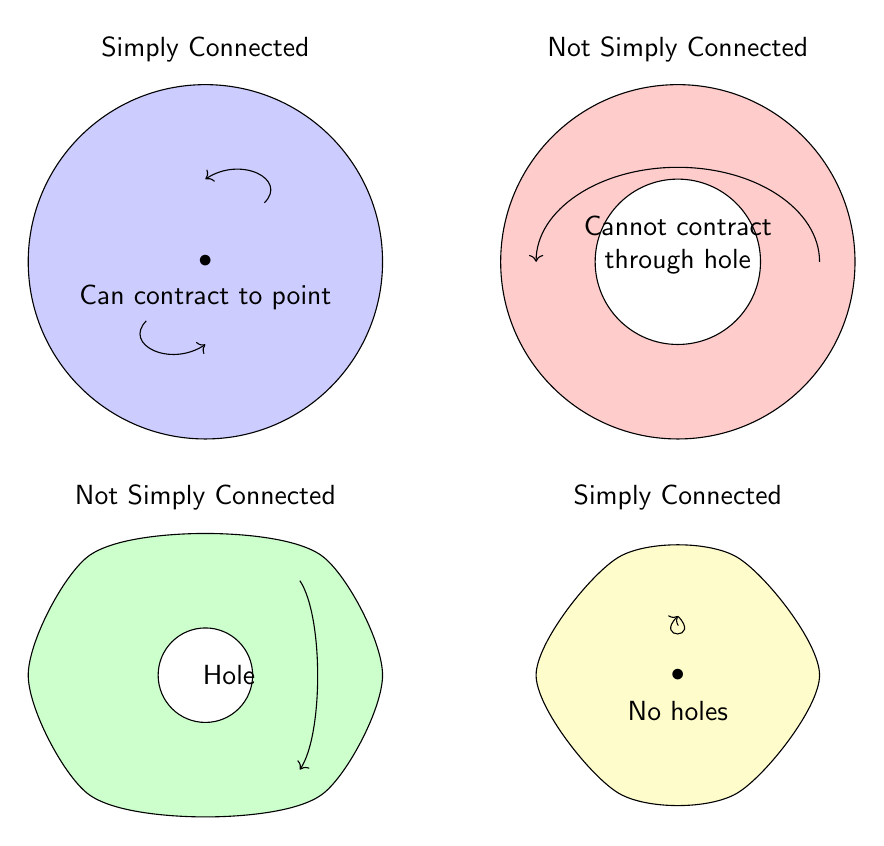
\begin{tikzpicture}[scale=1.5]
    
    % Simply connected domain (disk)
    \draw[fill=blue!20] (0,0) circle (1.5cm);
    \node at (0,1.8) {Simply Connected};
    \draw[->] (0.5,0.5) .. controls (0.7,0.7) and (0.3,0.9) .. (0,0.7);
    \draw[->] (-0.5,-0.5) .. controls (-0.7,-0.7) and (-0.3,-0.9) .. (0,-0.7);
    \node at (0,0) {$\bullet$};
    \node at (0,-0.3) {Can contract to point};
    
    % Non-simply connected domain (annulus)
    \begin{scope}[xshift=4cm]
    \draw[fill=red!20] (0,0) circle (1.5cm);
    \draw[fill=white] (0,0) circle (0.7cm);
    \node at (0,1.8) {Not Simply Connected};
    \draw[->] (1.2,0) arc (0:180:1.2cm and 0.8cm);
    \node at (0,0.3) {Cannot contract};
    \node at (0,0) {through hole};
    \end{scope}
    
    % Another non-simply connected example
    \begin{scope}[yshift=-3.5cm]
    \draw[fill=green!20] plot[smooth cycle] coordinates {(-1.5,0) (-1,1) (0,1.2) (1,1) (1.5,0) (1,-1) (0,-1.2) (-1,-1)};
    \draw[fill=white] (0,0) circle (0.4cm);
    \node at (0,1.5) {Not Simply Connected};
    \draw[->] (0.8,0.8) .. controls (1,0.5) and (1,-0.5) .. (0.8,-0.8);
    \node at (0.2,0) {Hole};
    \end{scope}
    
    % Simply connected but not convex
    \begin{scope}[xshift=4cm,yshift=-3.5cm]
    \draw[fill=yellow!20] plot[smooth cycle] coordinates {(-1.2,0) (-0.5,1) (0.5,1) (1.2,0) (0.5,-1) (-0.5,-1)};
    \node at (0,1.5) {Simply Connected};
    \draw[->] (0,0.5) .. controls (0.2,0.3) and (-0.2,0.3) .. (0,0.5);
    \node at (0,0) {$\bullet$};
    \node at (0,-0.3) {No holes};
    \end{scope}
    
    \end{tikzpicture}
    \end{figure}
\newpage
\section{Green's Theorem}
\subsection{Theorem}
Let $D \subseteq \mathbb{R}^2$ be open, and $v: D \to \mathbb{R}^2$ a continuously differentiable vector field. Furthermore, let $B \subseteq D \subseteq \mathbb{R}^2$ be a compact set (closed + bounded) with $\text{int}(B) \neq \emptyset$, and let $\text{bd}(B)$ consist of finitely many closed, piecewise smooth curves such that $B$ is to the left of these curves with respect to the direction of traversal of the respective curves. Then:

\[
\int_{\text{bd}(B)} v \, ds = \int_{B} \left( \frac{\partial v_2}{\partial x_1} - \frac{\partial v_1}{\partial x_2} \right) \, d(x_1, x_2).
\]

\subsection{Example*}
Consider the vector field:
\[
v \begin{pmatrix} x_1 \\ x_2 \end{pmatrix} = \begin{pmatrix} -x_2 \\ x_1 \end{pmatrix},
\]
and the set:
\[
B = \left\{ \begin{pmatrix} x_1 \\ x_2 \end{pmatrix} \in \mathbb{R}^2 : x_1^2 + x_2^2 \leq 7, \, x_2 \geq 0 \right\}.
\]

The boundary $\text{bd}(B)$ consists of two parts: $\gamma_1$ and $\gamma_2$, where:
\[
\gamma_1 : [-\sqrt{7}, \sqrt{7}] \rightarrow \mathbb{R}^2, \, \gamma_1(t) = \begin{pmatrix} t \\ 0 \end{pmatrix},
\]
\[
\gamma_2 : [0, \pi] \rightarrow \mathbb{R}^2, \, \gamma_2(t) = \begin{pmatrix} \sqrt{7} \cos t \\ \sqrt{7} \sin t \end{pmatrix}.
\]

\subsection{Application of Green's Theorem}
For the given vector field:
\[
\frac{\partial v_2}{\partial x_1} - \frac{\partial v_1}{\partial x_2} = 1 - (-1) = 2.
\]
Thus:
\[
\int_{B} \left( \frac{\partial v_2}{\partial x_1} - \frac{\partial v_1}{\partial x_2} \right) \, d(x_1, x_2) = \int_{B} 2 \, d(x_1, x_2) = 2 \cdot \text{vol}(B).
\]

On the other hand, the line integral over $\text{bd}(B)$ is:
\[
\int_{\text{bd}(B)} v \, ds = \int_{\gamma_1} v \, ds + \int_{\gamma_2} v \, ds.
\]

Calculating each part:
\[
\int_{\gamma_1} v \, ds = \int_{-1}^{1} \langle v(\gamma_1(t)), \dot{\gamma}_1(t) \rangle \, dt = \int_{-1}^{1} \langle (-0, t), (1, 0) \rangle \, dt = 0,
\]
\[
\int_{\gamma_2} v \, ds = \int_{0}^{\pi} \langle v(\gamma_2(t)), \dot{\gamma}_2(t) \rangle \, dt = \int_{0}^{\pi} \langle (-\sin t, \cos t), (-\sin t, \cos t) \rangle \, dt = \int_{0}^{\pi}  (\sin^2 t + \cos^2 t) \, dt = \pi.
\]

Therefore:
\[
2 \cdot \text{vol}(B) = \pi \implies \text{vol}(B) = \frac{\pi}{2}.
\]
\newpage
\textbf{Problem} \\
Consider the points \( a = (1,0) \) and \( b = (-1,0) \) in \(\mathbb{R}^2\).

\begin{enumerate}
    \item Determine a parameterization for the curve \(\gamma_1\) with endpoints \( a \) and \( b \) (starting at \( a \)) that corresponds to the straight line connecting these two points.
    
    \textbf{Solution:}
    The line connecting \( a \) and \( b \) can be parameterized as:
    \[
    \gamma_1(t) = t \cdot b + (1 - t) \cdot a = \begin{pmatrix} -2t + 1 \\ 0 \end{pmatrix}, \quad t \in [0, 1].
    \]

    \item Determine a parameterization for the curve \(\gamma_2\) with endpoints \( a \) and \( b \) (starting at \( a \)) that corresponds to a line along the unit circle with \( x_2 \geq 0 \) connecting these two points.
    
    \textbf{Solution:}
    The unit circle can be parameterized as:
    \[
    \gamma_2(t) = \begin{pmatrix} \cos(t) \\ \sin(t) \end{pmatrix}, \quad t \in [0, \pi].
    \]

    \item Consider the vector field \( v : \mathbb{R}^2 \rightarrow \mathbb{R}^2 \) given by:
    \[
    v(x_1, x_2) = \begin{pmatrix} x_1 \\ x_1^2 + x_2^2 \end{pmatrix}.
    \]
    Compute the line integrals of \( v \) along the curves \(\gamma_1\) and \(\gamma_2\).
    
    \textbf{Solution:}
    First, compute the derivatives of the parameterizations:
    \[
    \gamma_1'(t) = \begin{pmatrix} -2 \\ 0 \end{pmatrix}, \quad \gamma_2'(t) = \begin{pmatrix} -\sin(t) \\ \cos(t) \end{pmatrix}.
    \]
    The line integrals are:
    \[
    \int_{\gamma_1} v(x) \, dx = \int_{0}^{1} v(\gamma_1(t))^\top \gamma_1'(t) \, dt = \int_{0}^{1} (-2)(-2t + 1) \, dt = 0,
    \]
    \[
    \int_{\gamma_2} v(x) \, dx = \int_{0}^{\pi} \left( -\sin(t)\cos(t) + \cos(t) \right) dt = 0.
    \]

    \item Is \( v \) a conservative field?
    
    \textbf{Solution:}
    No, because the Jacobian matrix of \( v \):
    \[
    J_v(x_1, x_2) = \begin{pmatrix} 1 & 0 \\ 2x_1 & 2x_2 \end{pmatrix},
    \]
    is not symmetric. Thus, \( v \) is not conservative
    
\item 
\vspace{5mm}
Use Green's theorem to compute the integral of the vector field:
\[
v(x_1, x_2) = \begin{pmatrix} x_1 x_2 \\ x_1^2 x_2^3 \end{pmatrix},
\]
along the curve \(\gamma\) defined as the boundary of the triangle \( B \) with vertices \((0,0)^\top\), \((1,0)^\top\), and \((1,2)^\top\) (in counterclockwise direction).
\\
By Green's theorem:
\[
\int_{\gamma} v(x) \, dx = \int_{B} \left( \frac{\partial v_2}{\partial x_1} - \frac{\partial v_1}{\partial x_2} \right) d(x_1, x_2),
\]
where:
\[
\frac{\partial v_2}{\partial x_1} = 2x_1 x_2^3, \quad \frac{\partial v_1}{\partial x_2} = x_1.
\]
The integral becomes:
\[
\int_{B} (2x_1 x_2^3 - x_1) \, d(x_1, x_2) = \int_{0}^{1} \int_{0}^{2x_1} (2x_1 x_2^3 - x_1) \, dx_2 \, dx_1 = \frac{2}{3}.
\]

\item Consider the conservative vector field \( v: \mathbb{R}^{2} \to \mathbb{R}^{2} \) given by 
\[ v(x_{1}, x_{2}) = \begin{pmatrix} 2x_{1}x_{2} \cdot e^{x_{1}^{2} + x_{2}} \\ e^{x_{2}} \cdot \left(1 + e^{x_{1}^{2}} + x_{2} e^{x_{1}^{2}}\right) \end{pmatrix}. \]

\begin{enumerate}
    \item[a)] Determine an antiderivative \( F: \mathbb{R}^{2} \to \mathbb{R} \) of \( v \), i.e., a function with \( \nabla F(x) = v(x) \).

    \item[b)] Let \( \gamma \) be a curve in \( \mathbb{R}^{2} \) that starts at \( (1, 0) \) and ends at \( (0, 1) \). Determine the line integral \( \int_{\gamma} v(x) \, \mathrm{d}x \).
\end{enumerate}

\textbf{Solution}

\begin{enumerate}
    \item[a)] For an antiderivative \( F \) of \( v \), the following relations need to hold:
    \[
    \frac{\partial F}{\partial x_{1}}(x_{1}, x_{2}) = v_{1}(x_{1}, x_{2}) = 2x_{1}x_{2} \cdot e^{x_{1}^{2} + x_{2}}
    \]
    \[
    \frac{\partial F}{\partial x_{2}}(x_{1}, x_{2}) = v_{2}(x_{1}, x_{2}) = e^{x_{2}} \cdot \left(1 + e^{x_{1}^{2}} + x_{2} e^{x_{1}^{2}}\right)
    \]
    
    We can thus use successive integration to determine \( F \). First, we integrate \( v_{1}(x_{1}, x_{2}) \) with respect to \( x_{1} \) and obtain
    \[
    F(x_{1}, x_{2}) = \int v_{1}(x_{1}, x_{2}) \, \mathrm{d}x_{1} = \int 2x_{1}x_{2} \cdot e^{x_{1}^{2} + x_{2}} \, \mathrm{d}x_{1} = x_{2} \cdot e^{x_{1}^{2} + x_{2}} + G(x_{2}),
    \]
    where \( G \) is a function of \( x_{2} \) alone. Differentiating this result with respect to \( x_{2} \) yields
    \[
    \frac{\partial F(x_{1}, x_{2})}{\partial x_{2}} = e^{x_{1}^{2} + x_{2}} + x_{2} \cdot e^{x_{1}^{2} + x_{2}} + G'(x_{2}) = e^{x_{2}} \cdot \left(e^{x_{1}^{2}} + x_{2} e^{x_{1}^{2}}\right) + G'(x_{2}).
    \]
    
    Comparison with \( v_{2} \) now results in \( G'(x_{2}) = e^{x_{2}} \), so we get
    \[
    G(x_{2}) = \int G'(x_{2}) \, \mathrm{d}x_{2} = \int e^{x_{2}} \, \mathrm{d}x_{2} = e^{x_{2}} + C
    \]
    for a constant \( C \) and thus
    \[
    F(x_{1}, x_{2}) = x_{2} \cdot e^{x_{1}^{2} + x_{2}} + e^{x_{2}}
    \]
    as one possible antiderivative of \( v \) (we choose to set \( C = 0 \) here because the question only asks for one possible antiderivative of \( f \)).

    \item[b)] As \( v \) is conservative with antiderivative \( F \), the value of a line integral over \( v \) does not depend on the curve that connects the endpoints. Hence, we can easily compute the integral using
    \[
    \int_{\gamma} v(x) \, \mathrm{d}x = F(0, 1) - F(1, 0) = e^{1} + e^{1} - 0 - e^{0} = 2e - 1.
    \]
\end{enumerate}
\item 
An ellipse \( E(a; b) = \{(x_1, x_2) \in \mathbb{R}^2 : \left( \frac{x_1}{a} \right)^2 + \left( \frac{x_2}{b} \right)^2 \leq 1\} \) with semiaxes \( a \) and \( b \) (where \( a, b > 0 \)) can be considered as the image of two parameters, radius \( r \) and angle \( \phi \), under the transformation \( T : [0; 1] \times [0; 2\pi) \to \mathbb{R}^2 \) (elliptic polar coordinates) defined by
\[
T(r, \phi) = \begin{pmatrix}
a \cdot r \cos(\phi) \\
b \cdot r \sin(\phi)
\end{pmatrix}.
\]

\begin{enumerate}
    \item[a)] Compute the determinant of the Jacobian of \( T \).
    \item[b)] Use the elliptic polar coordinates defined by \( T \) above to compute the integral
    \[
    \int_{E(2,1)} x_1 \sqrt{\left( \frac{x_1}{2} \right)^2 + x_2^2} \, \mathrm{d}(x_1, x_2).
    \]
\end{enumerate}

\textbf{Solution}

\begin{enumerate}
    \item[a)] We start with the Jacobian of \( T \):
    \[
    J_{T}(r, \phi) = \begin{pmatrix}
    a \cdot \cos(\phi) & -a \cdot r \sin(\phi) \\
    b \cdot \sin(\phi) & b \cdot r \cos(\phi)
    \end{pmatrix}.
    \]
    
    Consequently, the determinant of the Jacobian of \( T \) is
    \[
    \det(J_{T}(r, \phi)) = a b r \cdot \cos^{2}(\phi) + a b r \sin^{2}(\phi) = a b r.
    \]

    \item[b)] For this part, we integrate over the elliptical area \( E(2,1) \), which means we use \( a = 2 \) and \( b = 1 \) for the parameter values. Using the transformation rule, we can compute the integral as follows:
    \[
    \int_{E(2,1)} x_{1} \sqrt{\left( \frac{x_{1}}{2} \right)^{2} + x_{2}^{2}} \, \mathrm{d}(x_{1}, x_{2})
    \]
    \[
    = \int_{E(2,1)} 2 \cdot r \cdot \cos(\phi) \cdot \sqrt{\left( \frac{2 \cdot r \cdot \cos(\phi)}{2} \right)^{2} + (1 \cdot r \cdot \sin(\phi))^{2}} \cdot 2 \cdot 1 \cdot r \, \mathrm{d}(r, \phi)
    \]
    \[
    = \int_{\phi=0}^{2\pi} \left( \int_{r=0}^{1} 2 r \cdot \cos(\phi) \cdot \sqrt{r^{2} \cos^{2}(\phi) + r^{2} \sin^{2}(\phi)} \cdot 2 r \, \mathrm{d}r \right) \, \mathrm{d}\phi
    \]
    \[
    = \int_{\phi=0}^{2\pi} \left( \int_{r=0}^{1} 2 r \cdot \cos(\phi) \cdot |r| \cdot 2 r \, \mathrm{d}r \right) \, \mathrm{d}\phi = \int_{\phi=0}^{2\pi} \left( \int_{r=0}^{1} 4 r^{3} \cdot \cos(\phi) \, \mathrm{d}r \right) \, \mathrm{d}\phi
    \]
    \[
    = \int_{\phi=0}^{2\pi} \left[ r^{4} \cdot \cos(\phi) \right]_{r=0}^{1} \, \mathrm{d}\phi = \int_{\phi=0}^{2\pi} \cos(\phi) \, \mathrm{d}\phi = \left[ \sin(\phi) \right]_{\phi=0}^{2\pi} = 0.
    \]
\end{enumerate}
\end{enumerate}
\vfill 
Sommersemester 2024 \\
Technische Universit\"at M\"unchen
\end{document}


